% === RDTs
\section{\todo{Resonance Driving Terms}}

Decapoles, due to their order, contribute to many RDTs. Indeed, 50 of them can be theoretically 
observed in simulations and measurements. In practice, the contributions of individual multipoles
become indistinguishable as many resonances or lines overlap, making it impossible to isolate
certain terms. Some resonances, described in~\cref{appendix:rdts}, are unique to certain multipoles
when considering no too high orders. Those resonances, provided that they are sufficiently strong
and the beam close to them, can be measured via their RDTs.

Of interest to the LHC Operation, is the RDT $f_{1004}$, driving the resonance $1Q_x - 4Q_y$.
It can be seen in the horizontal frequency spectrum at $-4Q_y$ with an amplitude dependence on
$J_y^2$. 
Figure~\cref{fig:decapoles:rdts:tune_diagram} shows a frequency
map~\cite{yannis_papaphilippou_detecting_nodate} of a simulation including decapolar field errors,
where their impact on the beam is easily noticeable. The \todo{red} particles evolving close to the
resonance are affected by it and are subject to large tune shifts. Eventually, those particles are 
lost when their amplitude becomes too large.

\begin{figure}[!htb]
    \centering
    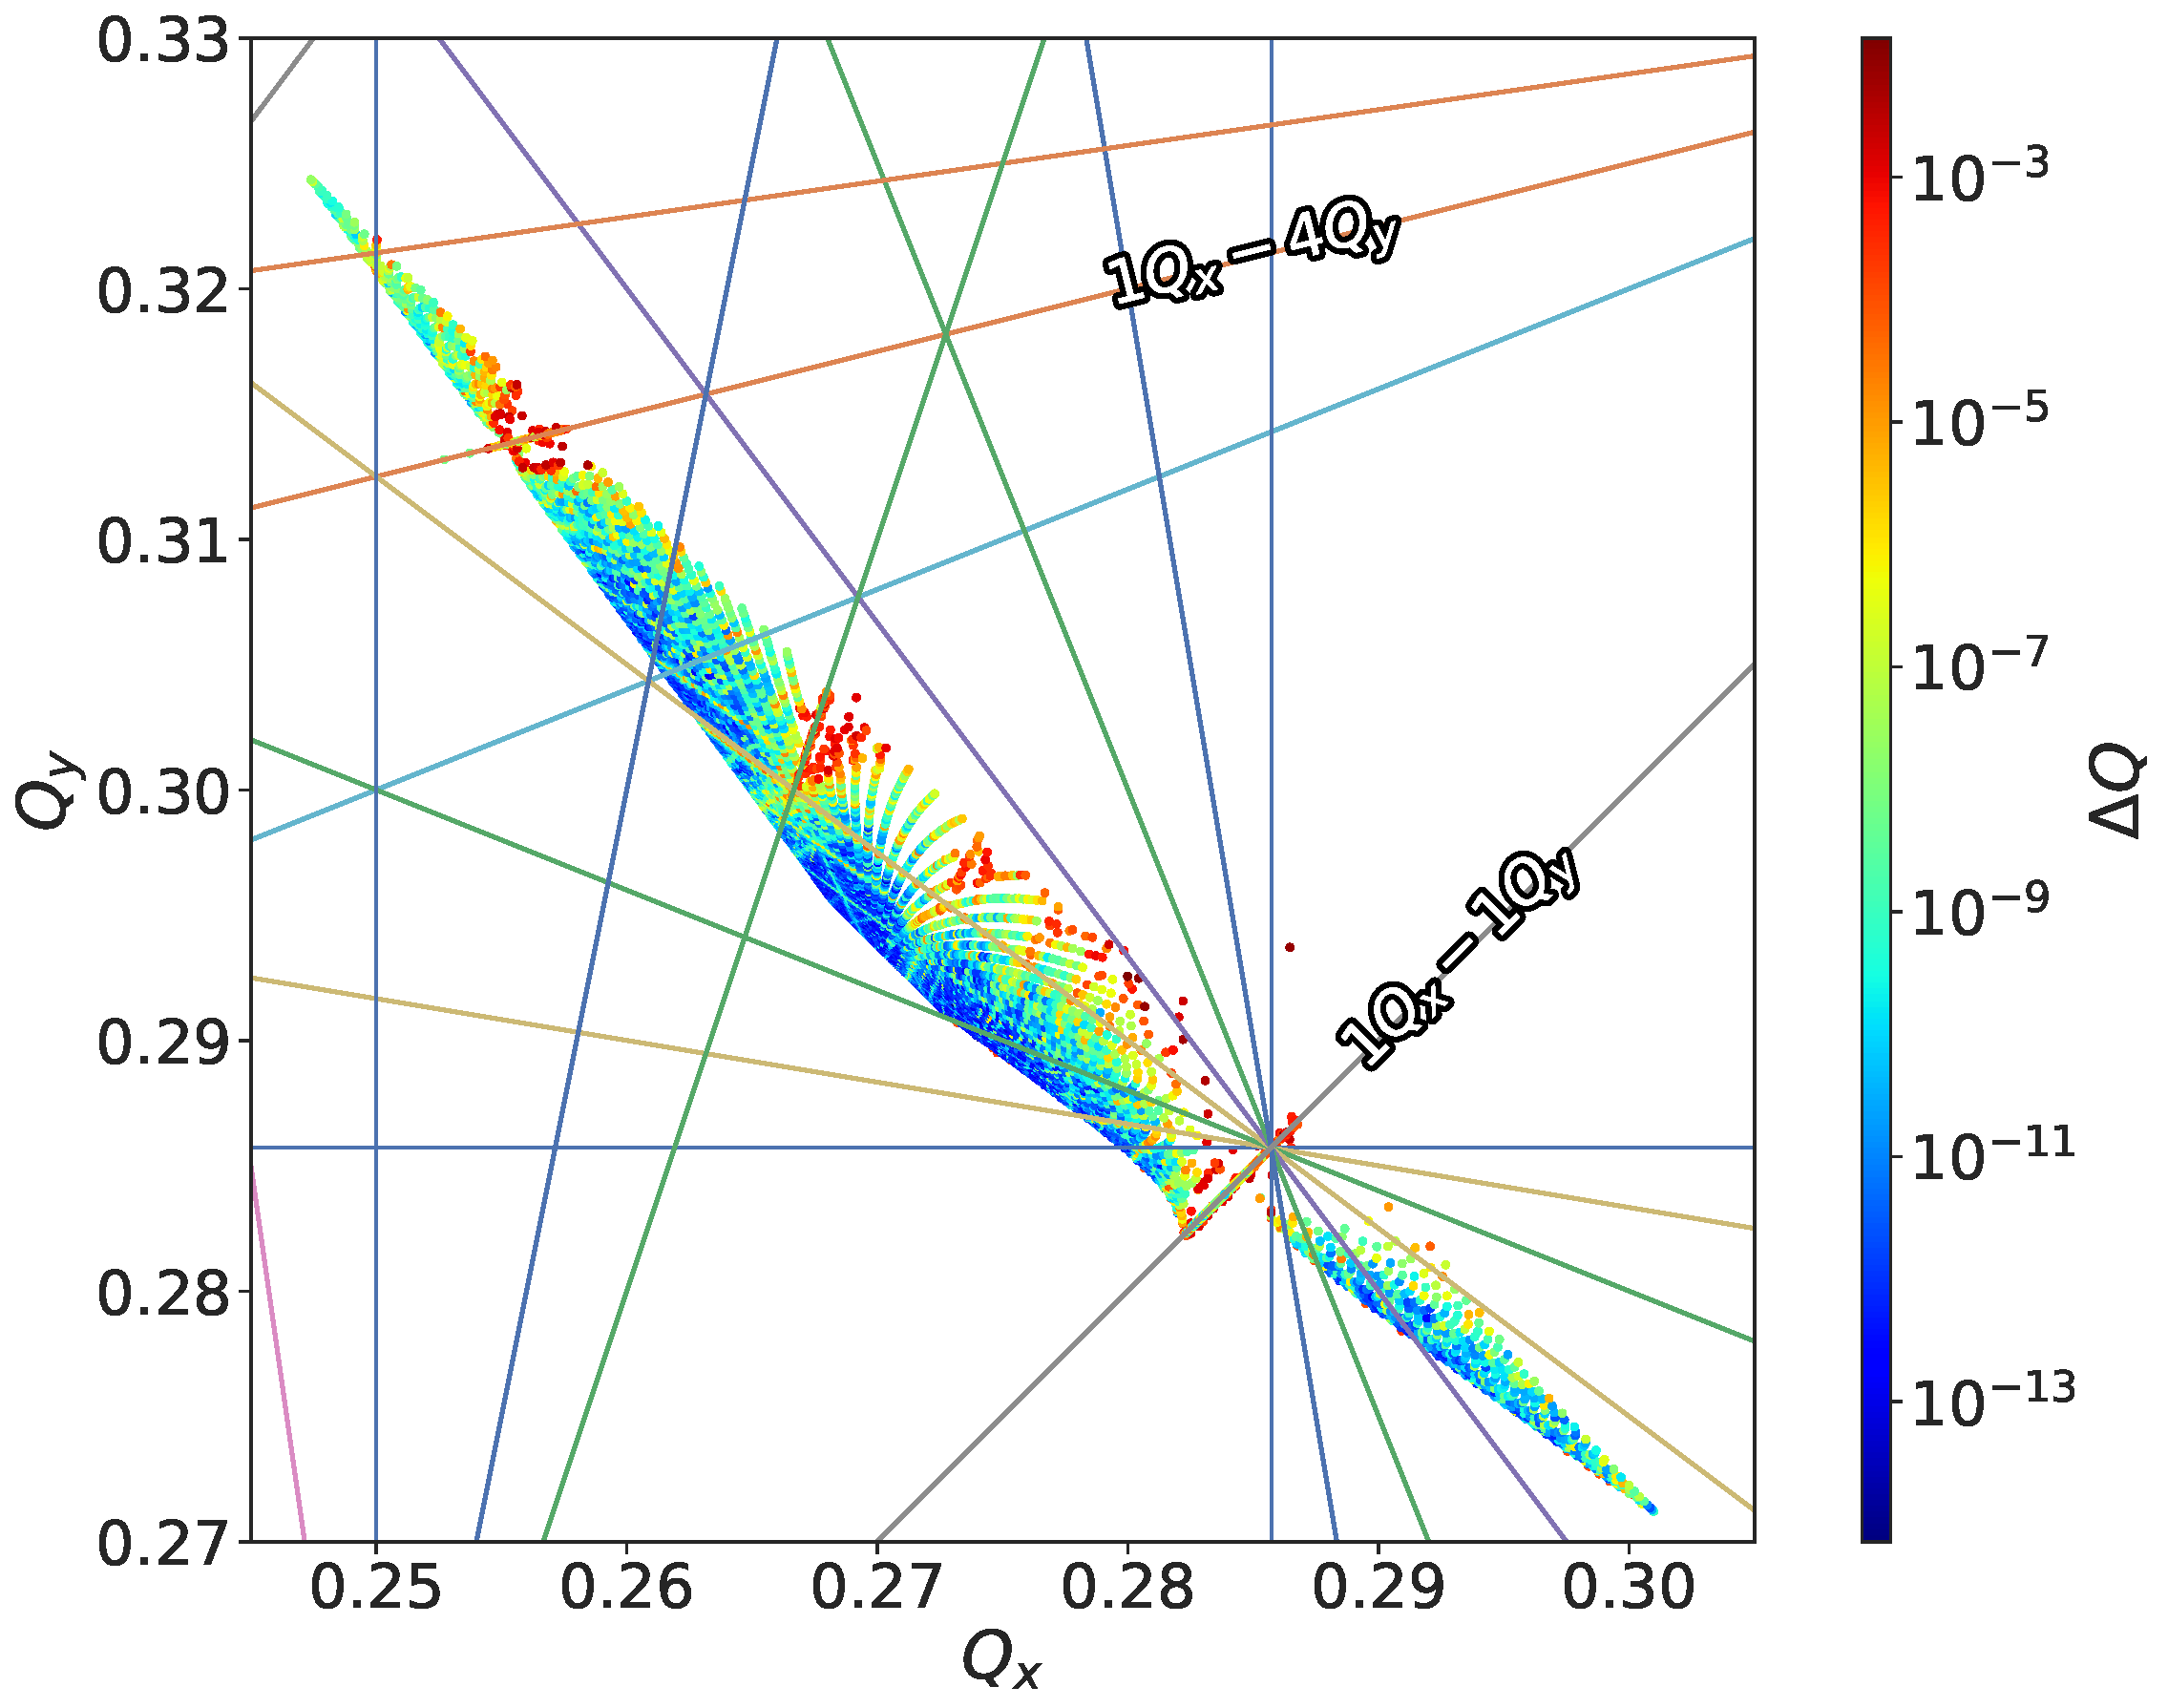
\includegraphics[width=0.8\textwidth]{./images/tune_diagram_f1004.pdf}
    \caption{Frequency map at injection energy, with decapolar field errors and nominal settings for
    landau octupoles. The highlighted resonance (1,-4), excited by decapoles, shows a degradation
    over 20,000 turns. The tune shift between the start and the end of the simulation is indicated
    in colour. \todo{change colormap}}
    \label{fig:decapoles:rdts:tune_diagram}
\end{figure}

Measuring turn-by-turn data without using any excitation is not a viable option as amplitudes are
not large enough. Spectral lines are indeed usually impossible to discern from the noise floor, 
making RDTs not measurable.
Measurements are hence taken with an AC-Dipole, introducing quadrupolar-like field errors in the 
linear regime~\cite{carlier_nonlinear_2020} and more complex effects in the non linear regime.
In practice, those effects are neglected. \textit{Forced} RDTs are measured with an
AC-Dipole and treated as \textit{free} as no compensation is applied.

Such forced measurements were taken for the first time in the LHC to observe the $f_{1004}$ RDT
at injection energy. The frequency line of the resonance $1Q_x - 4Q_y$ is seen at $4Q_y$ in the
horizontal spectrum, as shows \cref{fig:decapoles:rdts:spectrum_f1004}.

\begin{figure}[!htb]
    \centering
    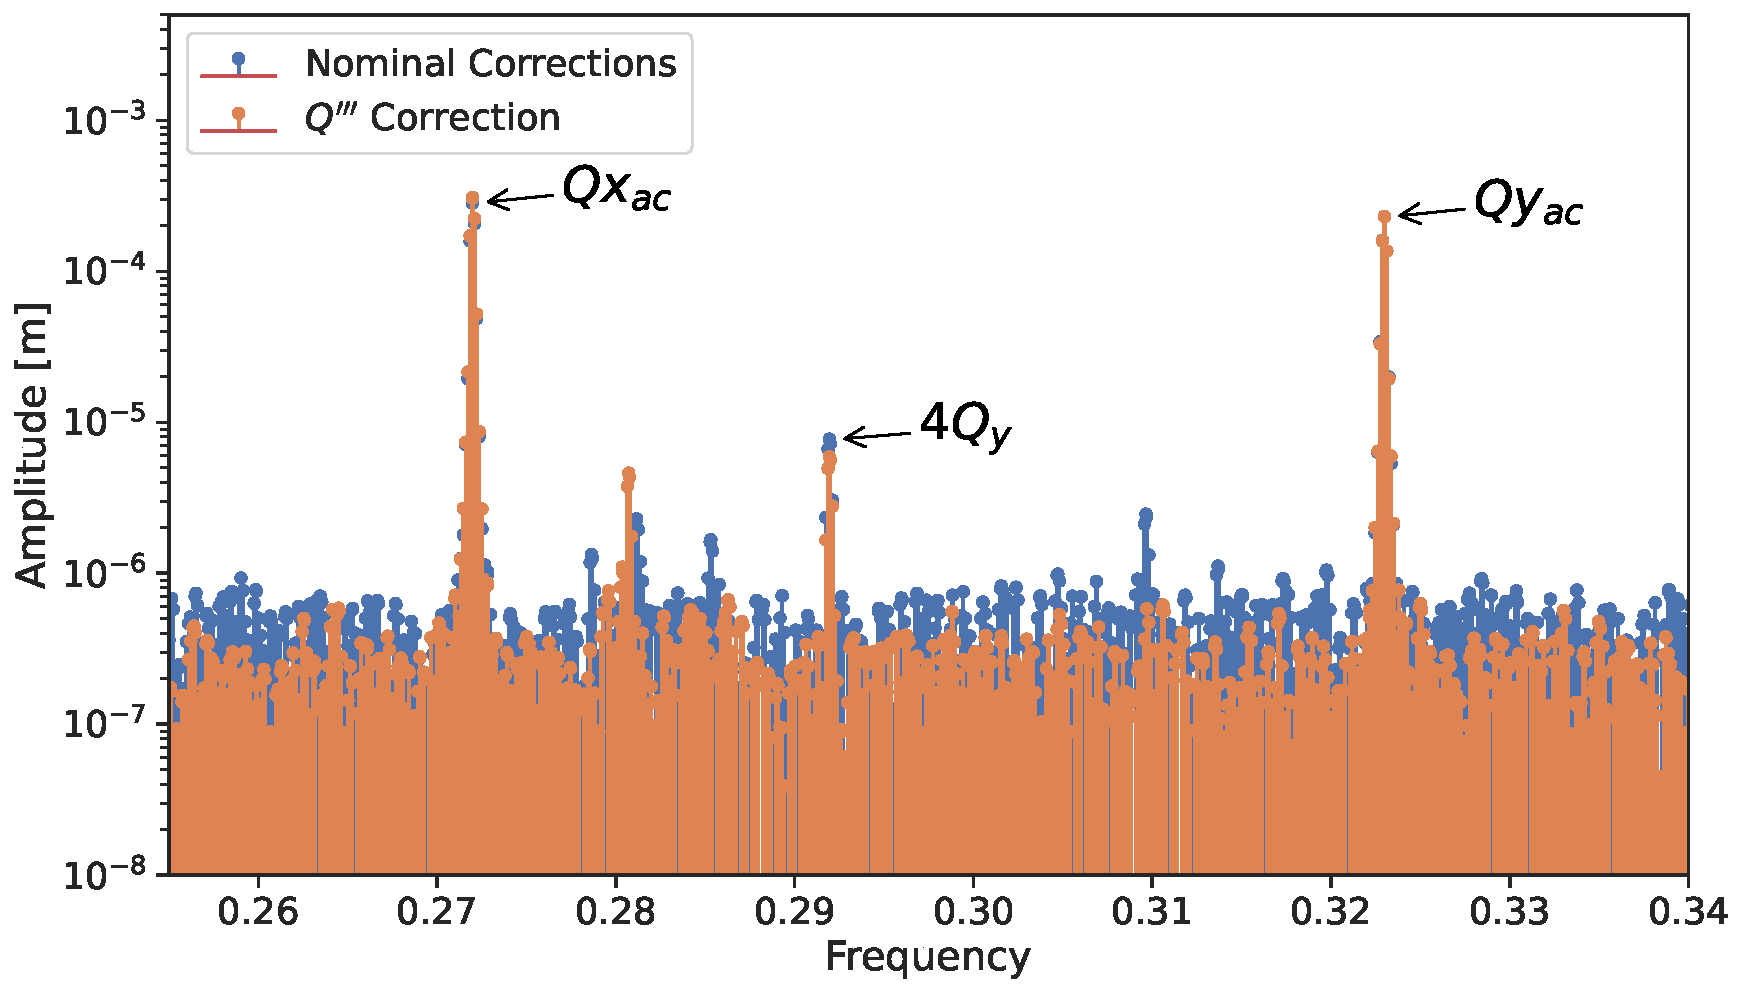
\includegraphics[width=0.9\textwidth]{./images/f1004x_spectrum.pdf}
    \caption{Horizontal frequency spectrum of turn-by-turn data, with nominal and beam-based
    corrections for the third order chromaticity $Q'''$. The $1Q_x - 4Q_y$ resonance can be seen
    at $-4Q_y$ with different amplitudes for each correction scheme.}
    \label{fig:decapoles:rdts:spectrum_f1004}
\end{figure}

%Moreover, \cref{fig:decapoles:rdts:spectrum_f1004} shows that the amplitude of this resonance line
%decreases upon application of beam-based corrections for $Q'''$. This translates to the amplitude
%of the RDT $f_{1004}$, as seen in \cref{fig:decapoles:rdts:f1004_dq3}.
%
%\begin{figure}[!htb]
%    \centering
%    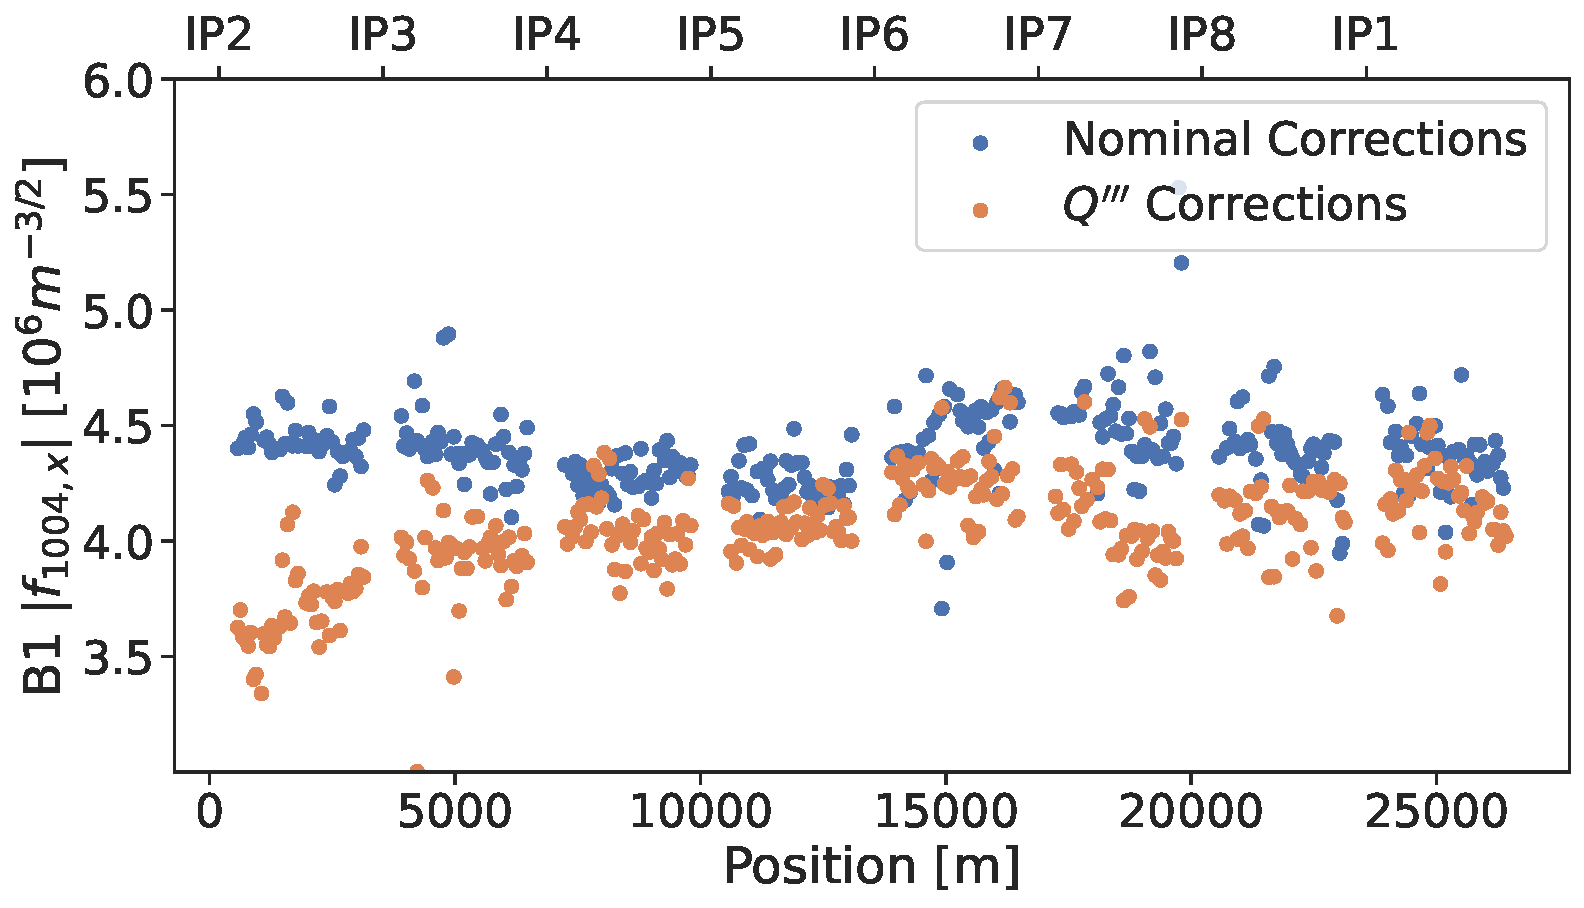
\includegraphics[width=0.9\textwidth]{./images/f1004_dq3.pdf}
%    \caption{Amplitude of the RDT $f_{1004}$ generated by normal decapoles, measured before and
%    after having applied beam-based corrections of the third order chromaticity $Q'''$.}
%    \label{fig:decapoles:rdts:f1004_dq3}
%\end{figure}

%\todo{
%    Measurements: \\
%    \begin{itemize}
%        \item 2022 Q'' and Q''' corrections 2022-04-24
%        \item 2022-10-19 Virgin machine
%        \item 2023-easter (FiDeL)
%        \item 2023-06-14 MD9549 (FiDeL and Q'''/ RDT corr)
%    \end{itemize}
%    Effect of RCO correction on RDT f1004 \\
%    Response
%}



% ---------------------------------------
%         Decapole Contribution
% ---------------------------------------
\subsection{\todo{Decapolar Contribution}}
\label{section:decapoles:decapolar_contribution_correction}

Decapolar fields are the main contributors to the RDT $f_{1004}$. As such, powering the decapolar
correctors is a good way to correct the related resonances.
Being linear with the strength of the correctors, the RDT can be corrected via a response matrix.

Measurements were taken in order to attempt such a correction and get a baseline for the amplitude
of the RDT without decapolar correctors and with the nominal FiDeL corrections applied.
Corrections were made on the base of those nominal settings and applied on top. The strength of the
decapolar correctors is shown in \cref{tab:decapoles:rdts:correction_f1004_k5} for the FiDeL
settings, the delta applied on top and the final correction values.


\begin{table}[!htb]
    \centering
    \begin{tabular}{lrrr}
    \toprule
    Circuit & FiDeL $K_5 [\textrm{m}^{-5}]$ & $\Delta K_5 [\textrm{m}^{-5}]$ & $K_5 [\textrm{m}^{-5}]$\\
    \midrule
    Beam 1 & \\
    \hspace{2mm}RCD.A12B1 &$-4582$ & $6055 $ &  $ 1473 $\\
    \hspace{2mm}RCD.A23B1 &$-5106$ & $7    $ &  $-5099 $\\
    \hspace{2mm}RCD.A34B1 &$-4855$ & $3827 $ &  $-1028 $\\
    \hspace{2mm}RCD.A45B1 &$-4577$ & $-4746$ &  $-9323 $\\
    \hspace{2mm}RCD.A56B1 &$-4125$ & $-4903$ &  $-9028 $\\
    \hspace{2mm}RCD.A67B1 &$-5166$ & $2961 $ &  $-2205 $\\
    \hspace{2mm}RCD.A78B1 &$-6827$ & $3593 $ &  $-3234 $\\
    \hspace{2mm}RCD.A81B1 &$-5500$ & $2380 $ &  $-3120 $\\
    \hspace{2mm}Total     &$-40738$& $9174 $ &  $-31564$\\
    Beam 2 & \\  % inverted the signs of the correction
    \hspace{2mm}RCD.A12B2 &$-4490$ & $3639 $ &  $-851  $\\
    \hspace{2mm}RCD.A23B2 &$-5155$ & $-1147$ &  $-6302 $\\
    \hspace{2mm}RCD.A34B2 &$-4825$ & $-1038$ &  $-5863 $\\
    \hspace{2mm}RCD.A45B2 &$-4619$ & $3986 $ &  $-633  $\\
    \hspace{2mm}RCD.A56B2 &$-4064$ & $2944 $ &  $-1120 $\\
    \hspace{2mm}RCD.A67B2 &$-5066$ & $2357 $ &  $-2709 $\\
    \hspace{2mm}RCD.A78B2 &$-6866$ & $-2952$ &  $-9818 $\\
    \hspace{2mm}RCD.A81B2 &$-5446$ & $1825 $ &  $-3621 $\\
    \hspace{2mm}Total     &$-40531$& $9614 $ &  $-30917$      \\
    \bottomrule
    \end{tabular}
    \caption{Strength of decapolar correctors with nominal FiDeL settings and after application of
    corrections aiming at reducing both the RDT $f_{1004}$ and $Q'''$. The total value as a direct
    incidence on the chromaticity}
    \label{tab:decapoles:rdts:correction_f1004_k5}
\end{table}

This RDT correction also serves as a partial $Q'''$ correction. To fully correct $Q'''$ indeed
approximately requires a strength of $+13,000 K_5$ distributed amongst the correctors. Therefore,
this new approach reduces $Q'''$ by about $70\%$ compared to the previous method. The chromatic
amplitude detuning terms are also expected to be decreased.
Result of those measurements, as well as the inverse of the correction, are shown in 
\cref{fig:decapoles:rdts:f1004_correction_B2}

\begin{figure}[!h]
    \centering
    \begin{subfigure}{1\textwidth}
        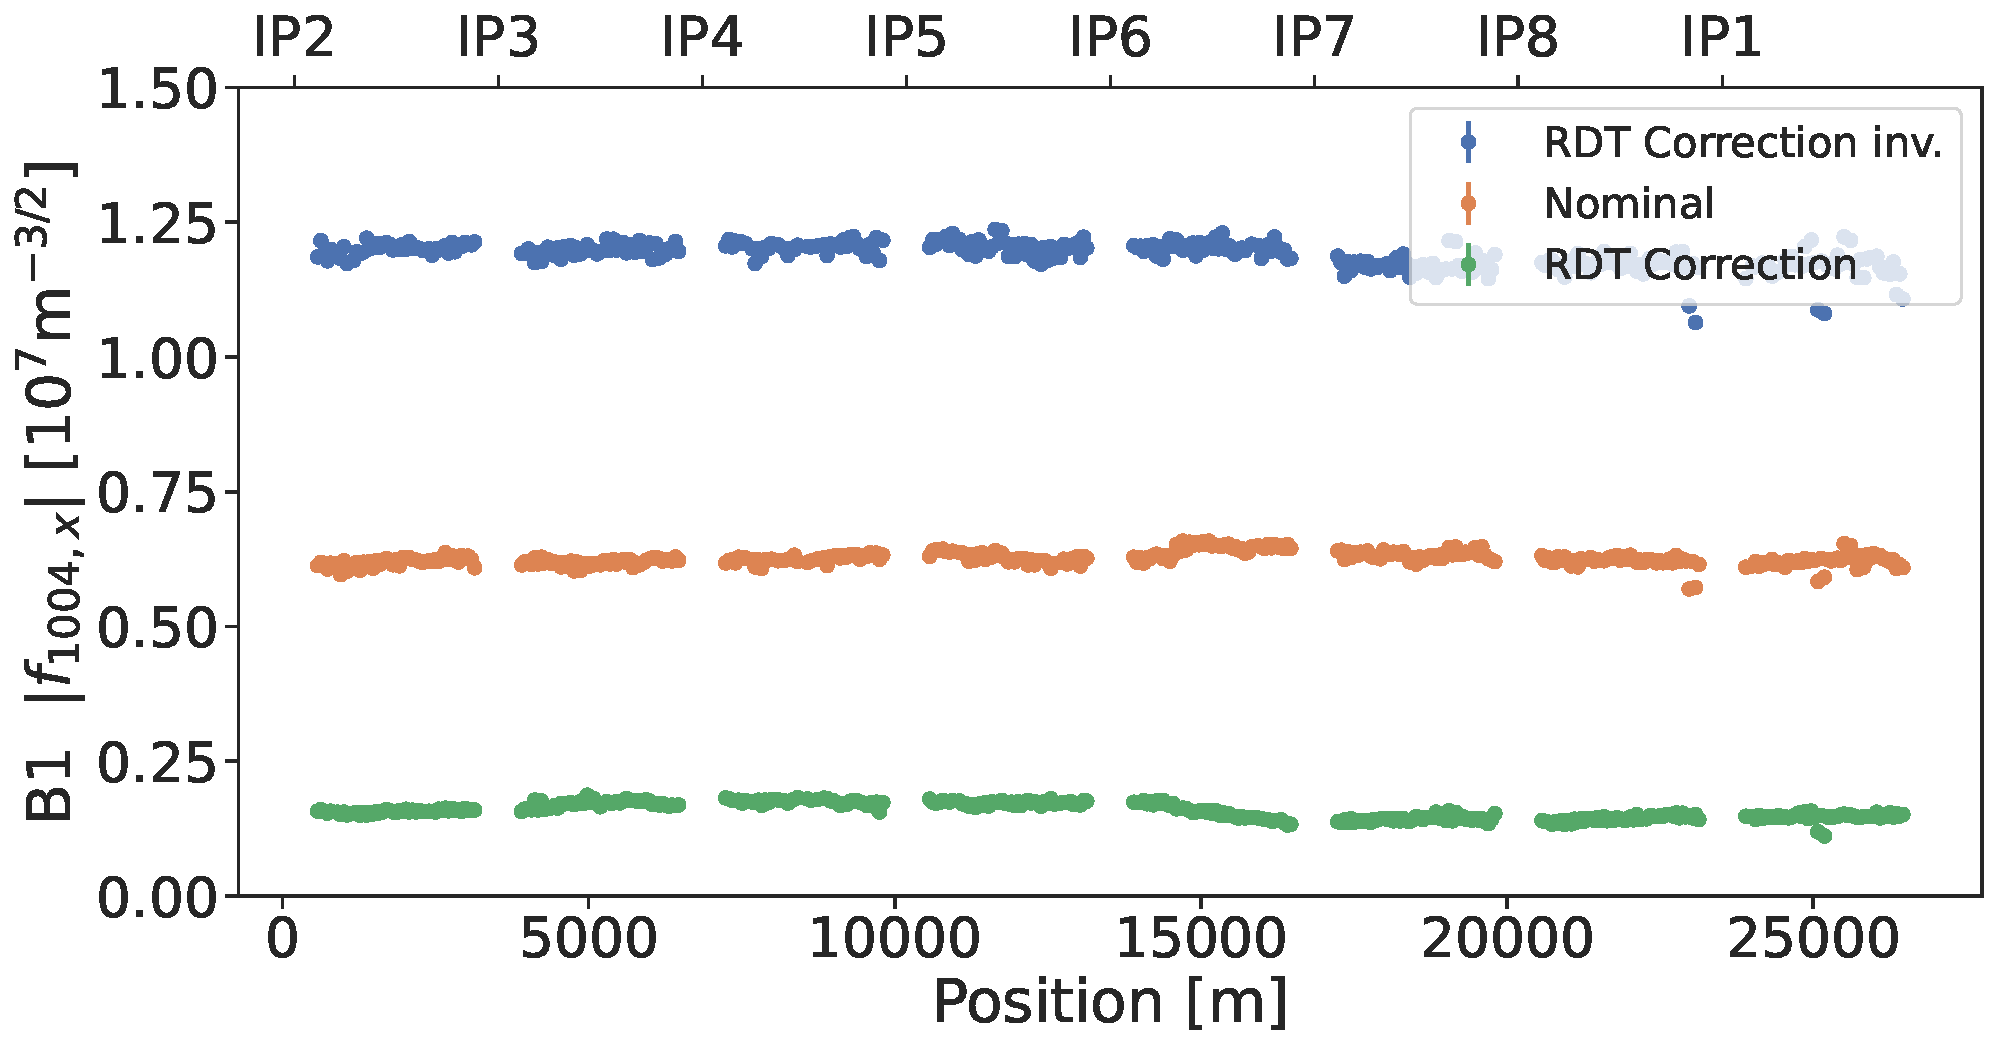
\includegraphics[width=0.9\textwidth]{./images/f1004/f1004x_corrections_B1.pdf}
        \caption{$|f_{1004}|$ for Beam 1}
        \vspace{0.5cm}
    \end{subfigure}
    \begin{subfigure}{1\textwidth}
        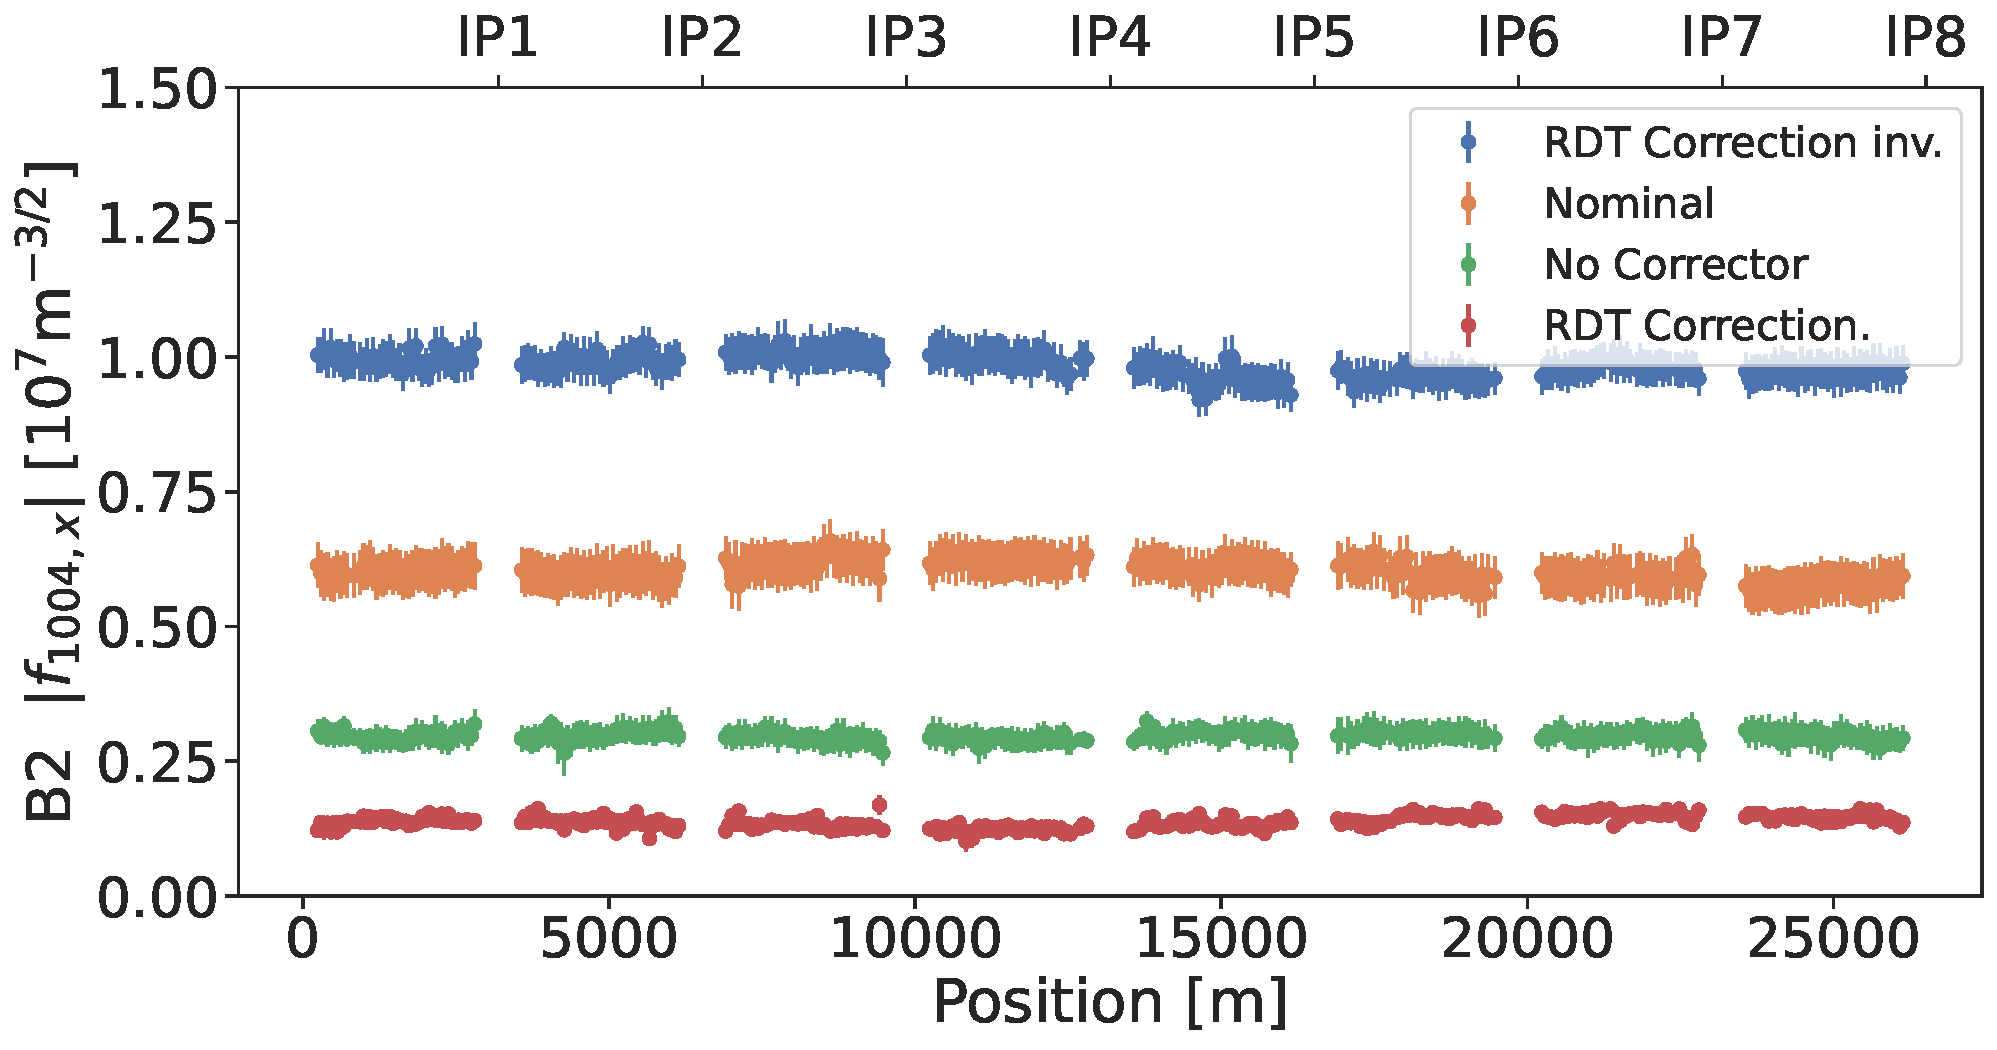
\includegraphics[width=0.9\textwidth]{./images/f1004/f1004x_corrections_B2.pdf}
        \caption{$|f_{1004}|$ for Beam 2}
    \end{subfigure}
    \caption{Measured $f_{1004}$ with decapolar correctors powered off, nominal settings, and
    combined RDT \& $Q'''$ correction with normal and opposite signs.}
    \label{fig:decapoles:rdts:f1004_correction_B2}
\end{figure}


Although the FiDeL scheme was not intended to correct the RDT but rather only $Q'''$, it would be 
expected for it to lower the amplitude of the RDT. It can though be seen that it degrades the
resonance compared to the machine with no decapolar correctors. On the other hand, the newly
computed RDT correction does lower the amplitude of $f_{1004}$ as expected.  Its inverse has the
opposite effect.

Simulations were run with decapolar correctors turned of and with the absolute value of the RDT
correction. The response of the RDT between those two schemes is shown in 
\cref{fig:decapoles:rdt:b1_response_corr}. The difference between their RMS value ratio is $\approx
6\%$, indicating that simulations correctly model the decapolar correctors.

\begin{figure}[!htb]
    \centering
    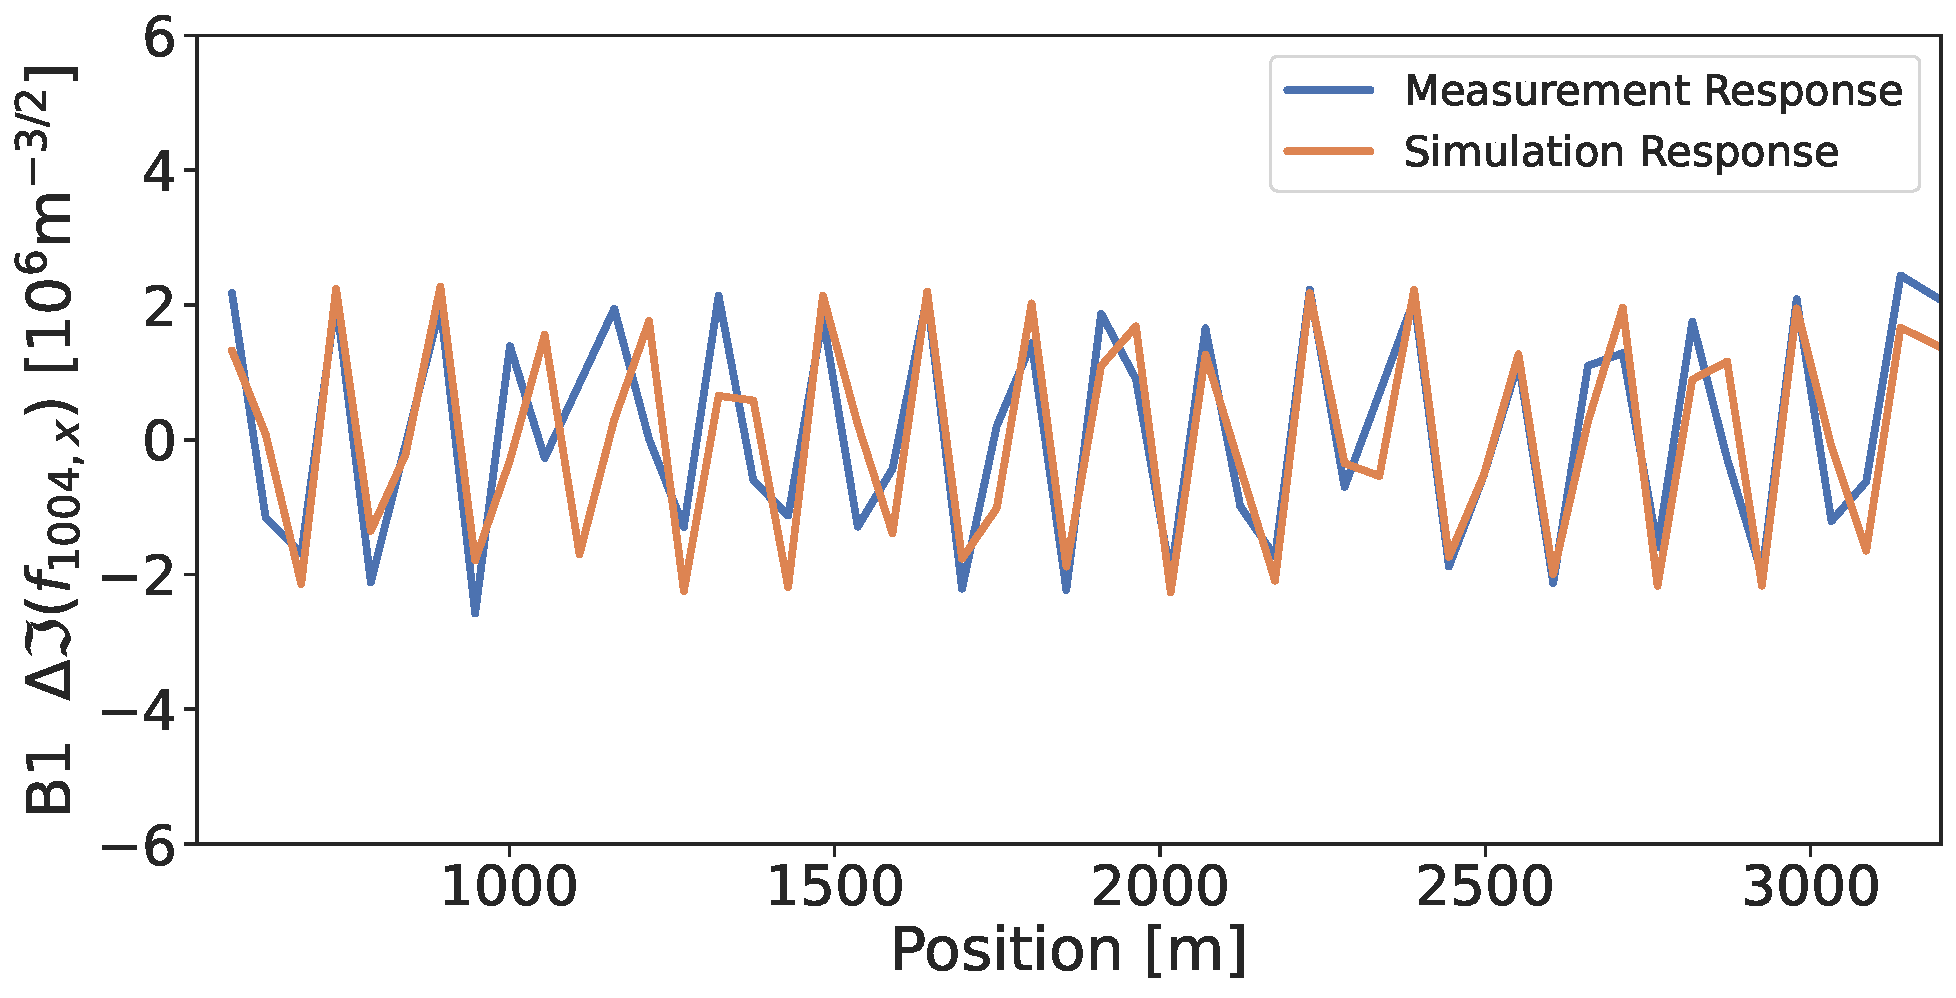
\includegraphics[width=0.9\textwidth]{./images/f1004/b1_response_rdt_corr.pdf}
    \caption{Comparison for measurement and simulation of the response of the imaginary part of
    $f_{1004}$ upon application on unpowered correctors of the RDT corrections.}
    \label{fig:decapoles:rdt:b1_response_corr}
\end{figure}


% ---------------------------------------
%        Higher Order Contribution
% ---------------------------------------
\subsection{\review{Higher Order Contributions}}

% Measurements in 
% /afs/cern.ch/work/m/mlegarr2/public/beta_beat_output/2024-05-21

To produce collisions at top energy, \textit{crossing angles} are introduced via the orbit
correctors located in the triplets, before the separation dipoles and the matching section of the
interaction regions (\texttt{MCBX}, \texttt{MCBY} and \texttt{MCBC})~\cite{de_maria_lhc_2008}. Those
collisions happen with a small $\beta*$, currently 30cm, requiring strong quadrupolar fields from
the triplets.

At such $\beta$, those triplets also generate strong dodecapolar field errors. Because of the
crossing-angles, feed-down appears and lower-order fields can be observed.
Such feed-down to decapolar fields was observed during the first commissioning of Run~3, in
2022~\cite{maclean_prospects_2022}.
\cref{fig:decapoles:f1004_from_feeddown} shows how the RDT $f_{1004}$, normally affected by
decapoles, varies with the application of crossing angles.

\begin{figure}[!htb]
    \centering
    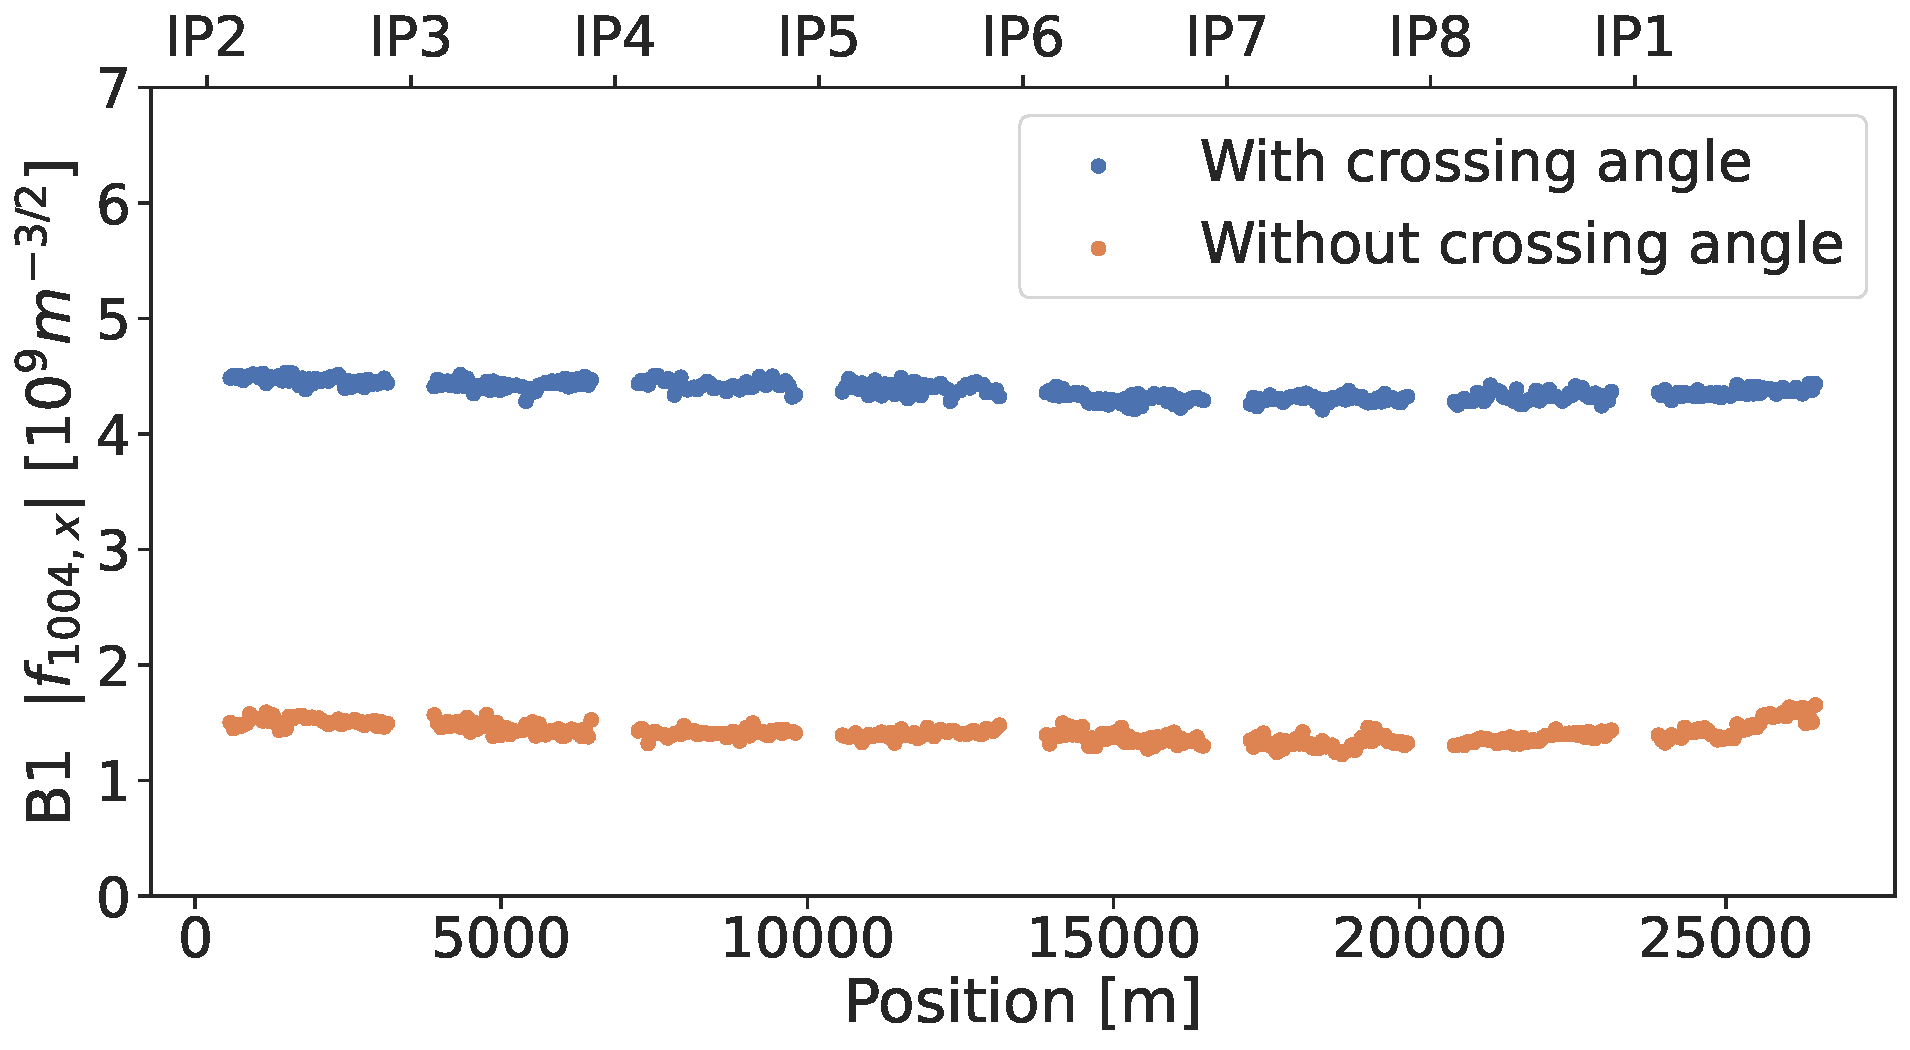
\includegraphics[width=0.9\textwidth]{./images/f1004x_feed-down_b6_triplets.pdf}
    \caption{Varying amplitude of the decapolar RDT $f_{1004}$ depending on the activation or not of
    the crossing angle at the IP. Offsets in orbit create feed-down from higher orders.}
    \label{fig:decapoles:f1004_from_feeddown}
\end{figure}

Such a contribution is though not expected at injection energy, as the triplets aren't powered as
much as at top energy, $\beta*$ being set at around $10$m.

% ---------------------------------------
%        Lower Order Contribution
% ---------------------------------------
\subsection{\review{Lower Order Contributions}}

% http://localhost:8888/lab/workspaces/auto-d/tree/work_afs2/jupyter/resonance_driving_terms/measurements/2024-03-13_b3_b4_effect_on_b5/Sextupoles_and_Octupoles.ipynb

% ------- Introduction
\subsubsection{\review{First Observation}}

As described in \cref{appendix:transfer_maps}, multipoles can combine to create fields that are seen
as higher orders when considering higher orders of the BCH expansion.
For decapoles, combinations of several sextupoles and sextupoles with octupoles give rise to
decapolar-like fields, as described in
\cref{table:appendix:transfer_maps:bch_resulting_orders_combination}. The following parts of this
section will describe those combinations.

This effect was observed in 2022 during Run 3's commissioning. New corrections of the non-linear
chromaticity $Q''$ and $Q'''$ were performed, and RDT measurements taken before and after their
correction. As $Q'''$ was corrected, the expectation was that the RDT $f_{1004}$ would also lower
with the reduction of the decapolar strengths $K_5$. However, an increase of the RDT was observed,
as shows \cref{fig:decapoles:f1004_dq2_dq3}.

\begin{figure}[H]
    \centering
    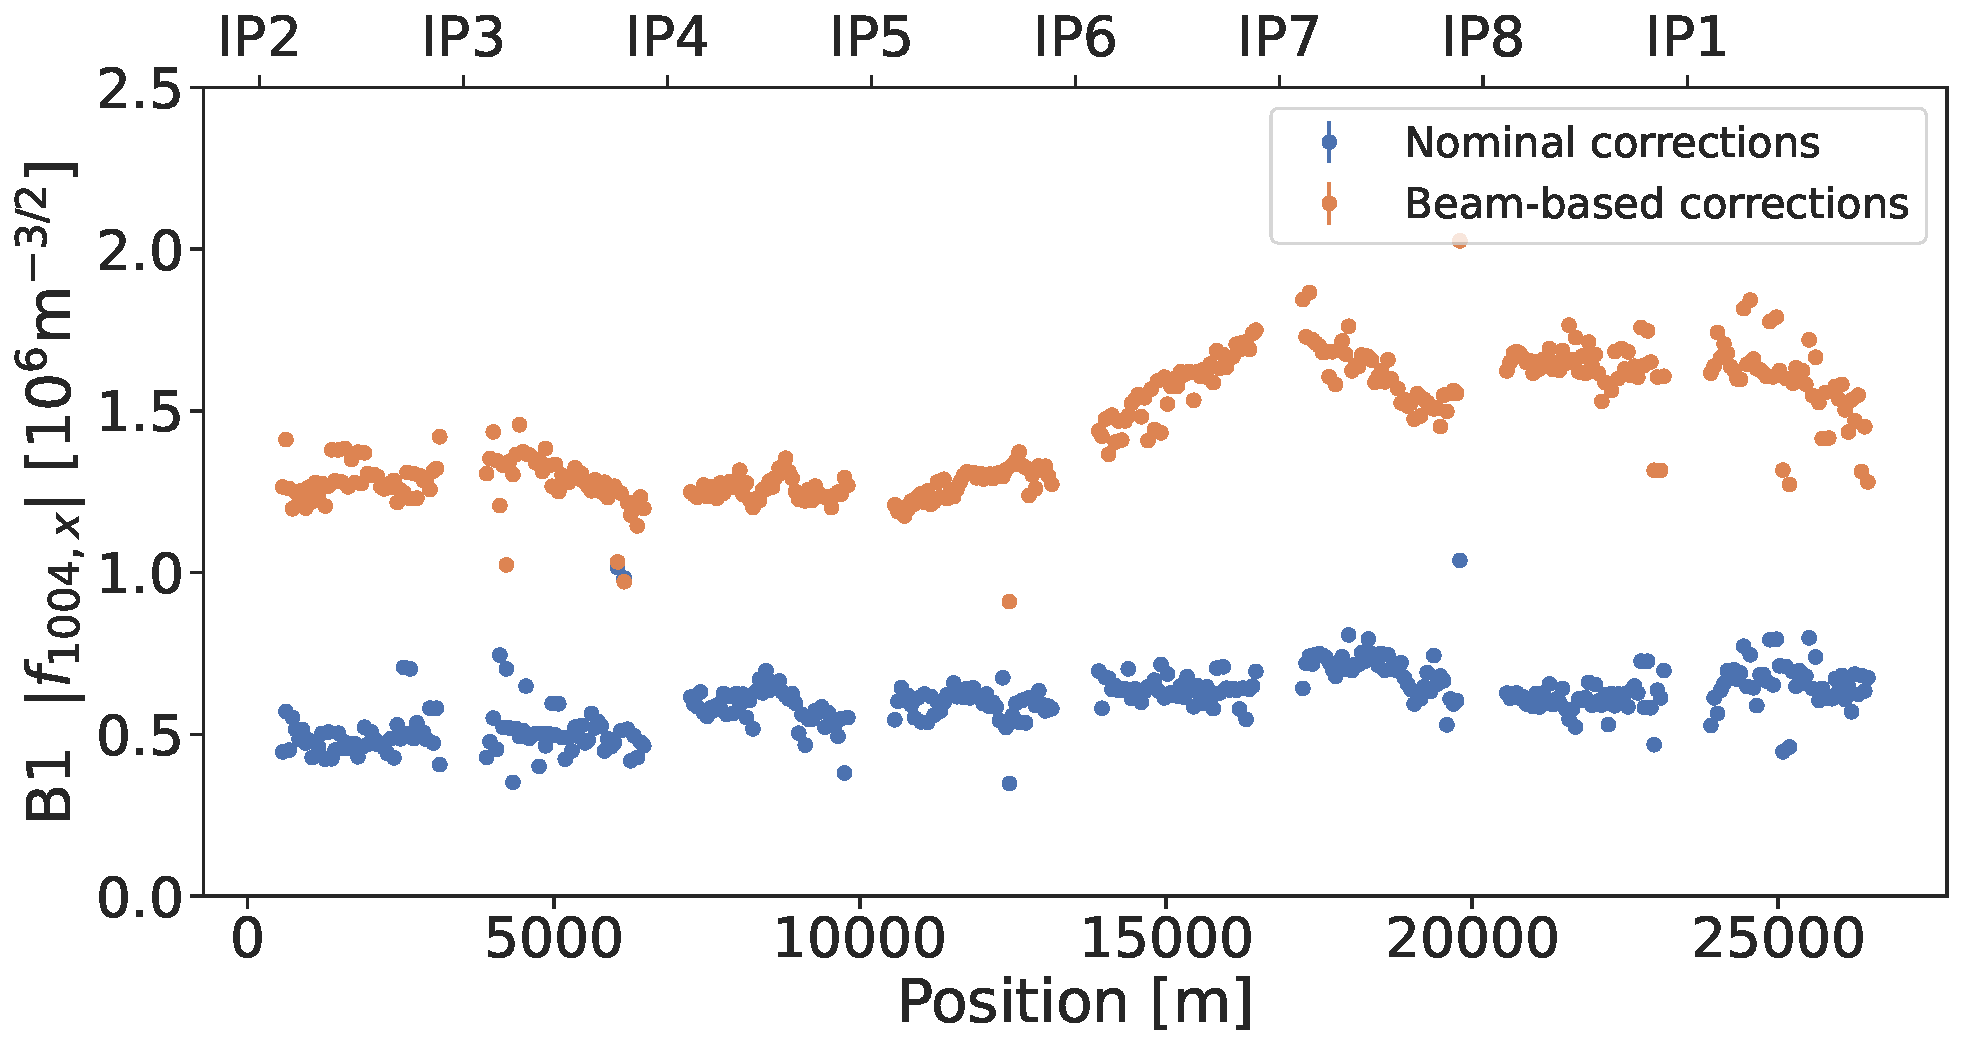
\includegraphics[width=0.9\textwidth]{./images/f1004_dq2_dq3_2022.pdf}    
    \caption{Non intuitive increase of the RDT $f_{1004}$ after application of both the $Q''$ and
    $Q'''$ corrections.\todo{redo plot}}
    \label{fig:decapoles:f1004_dq2_dq3}
\end{figure}


% ------- Action dependance
\subsubsection{\review{Action Dependance and Analysis}}

Resonance lines in the frequency spectrum are often contributed to by several multipoles. Some lines
start getting a contribution with rather high multipole orders, like the RDT $f_{1004}$ considered
here. The line $4Q_y$ in the horizontal spectrum is indeed contributed to by decapoles and then only
by decatetrapoles. When the main contributing field alone is varied, it is easy to reconstruct the
RDT, as its fit is only dependant its action dependance ($\propto J_x^{*} J_y^{*}$). Several
turn-by-turn measurements at the same configuration can be taken wit varying kick amplitudes,
refining the RDT value with more data points for the fit.

Considering the contribution of lower order multipoles is a bit trickier, as the second order RDTs
change the dependance of the frequency line~\cite{franchi_first_2014}. In order to be able to
compare the RDT from several turn by turn measurements, the same kick amplitude must then be used.
Failing to do so would lead to a poor fit of the line amplitude relative to the action, resulting in
an RDT with incorrect amplitude and significant noise.

%\todo{simulation plot of varying amplitudes for Q' = 2 and noise created from it}


% ------- Sextupoles ----------
\subsubsection{\review{Sextupoles}}

At the third order of the BCH expansion, the combination of two sextupoles yields a decapolar-like
expression. This means that, during normal operation of the machine, decapolar observables will be
altered when adjusting parameters such as the linear chromaticity $Q'$. 
Derivation of such a combination can be found in \cref{appendix:transfer_map:two_sextupoles}. The
resulting Hamiltonian indeed is similar to the terms of a decapole, dropping the $p_{x,y}$ terms for
readability:

\begin{equation}
    \begin{aligned}
         (H_3)^3 &\propto \frac{1}{48} \left(x^5 - 2x^3y^2 - 3xy^4 \right)\\
                 &\sim    x^5 - 10x^3y^2 + 5xy^4.
    \end{aligned}
    \label{eq:decapoles:sextupoles_b5}
\end{equation}

To quantify the actual impact of such an equation on the LHC, a simulation was run with injection
optics while varying this same linear chromaticity $Q'$. No higher fields than sextupoles are 
have been included, including field errors. The resulting effect on the RDT $f_{1004}$
can be seen in \cref{fig:decapoles:rdts:simulated_f1004_from_sextupoles}.

\begin{figure}[H]
    \centering
    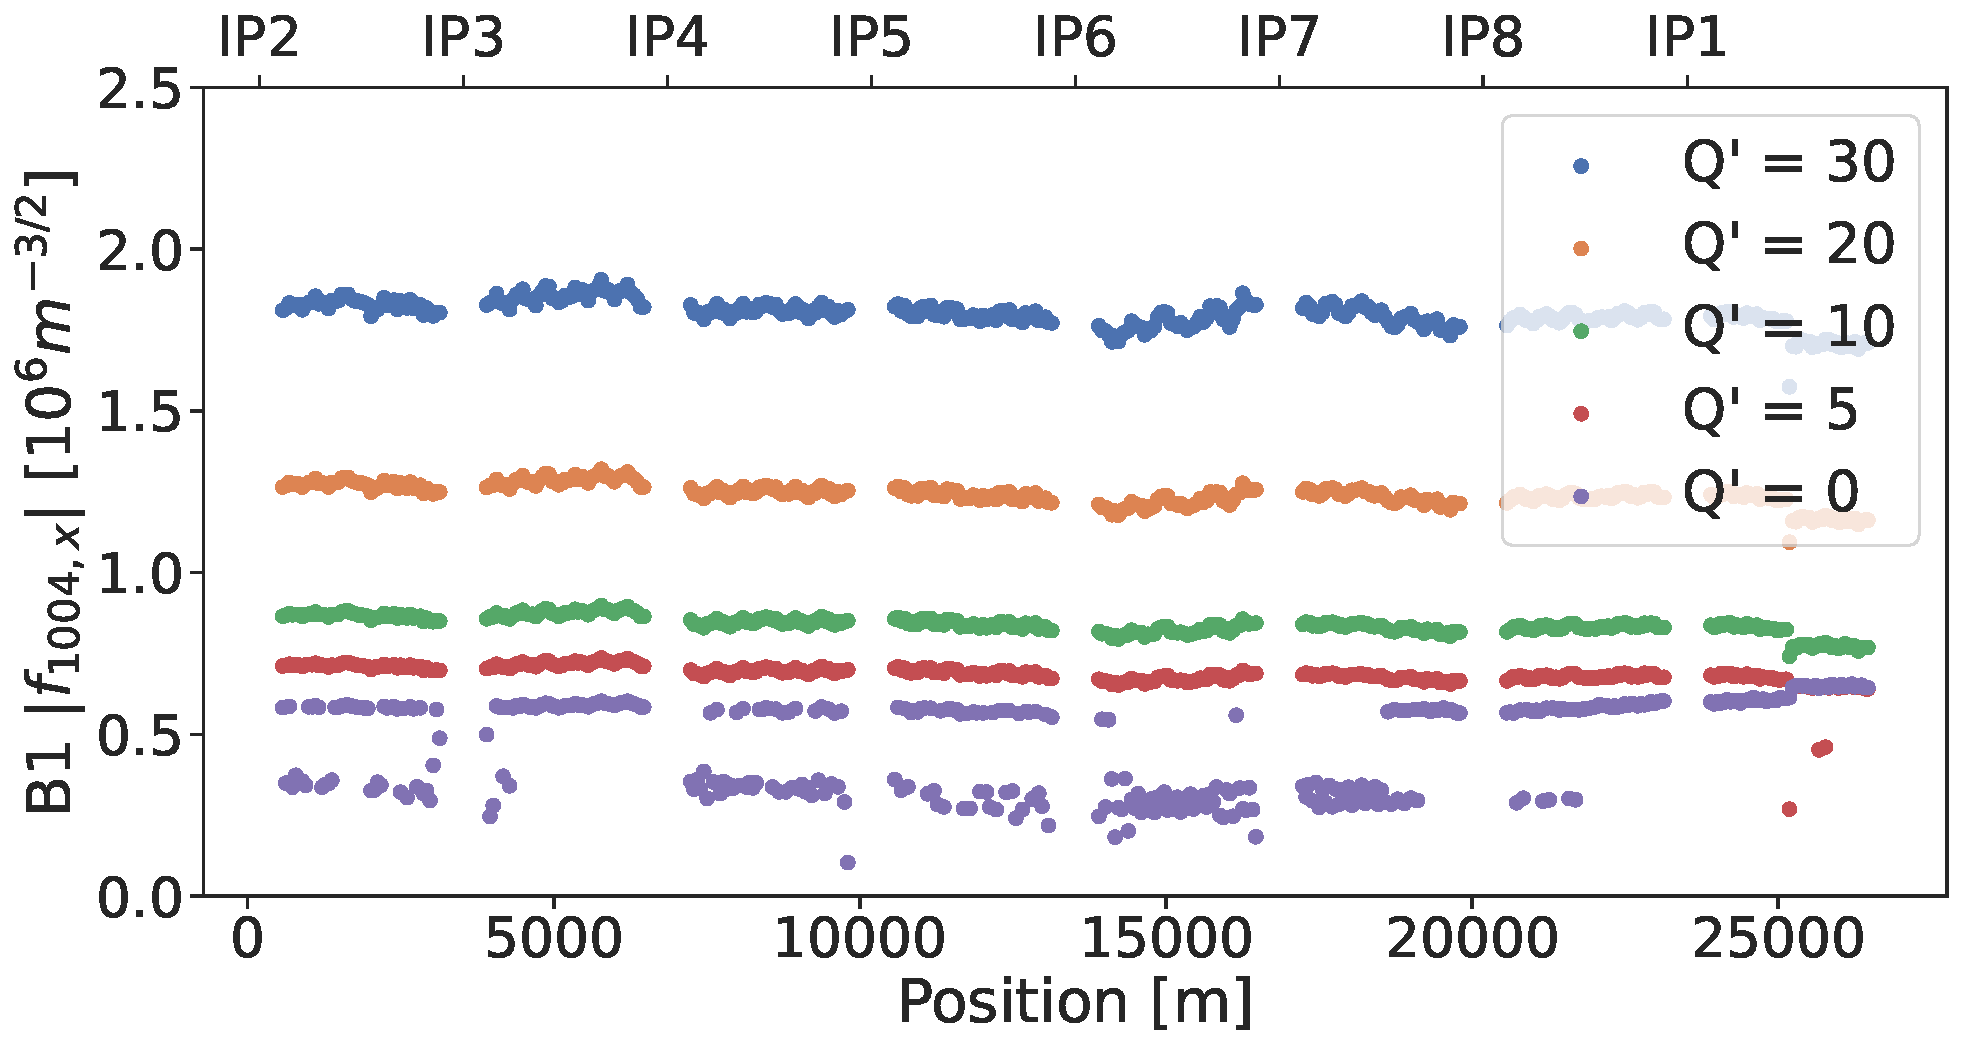
\includegraphics[width=0.7\textwidth]{./images/f1004/f1004_dq.pdf}
    \caption{Simulated change of the decapolar RDT $f_{1004}$ with varying linear
    chromaticity $Q'$ generated by sextupoles. The combination of sextupolar fields clearly shows a 
    increase in decapolar RDT.}
    \label{fig:decapoles:rdts:simulated_f1004_from_sextupoles}
\end{figure}

As the linear chromaticity increases, the overall $K_3$ strength of sextupoles actually becomes 
more negative. Considering the previous \cref{eq:decapoles:sextupoles_b5}, a higher chromaticity
is expected to increase the amplitude of the RDT $f_{1004}$, related to the last term $xy^4$.
\cref{fig:decapoles:sextupoles_k3_f1004} shows how the RDT is expected to vary, depending on the
overall sextupoles strength and the linear chromaticity. It can be noted that although the relation
between $K_3$ and $Q'$ is linear, that of $K_3$ and the RDT varies with the cubed strength. Using 
the sum of the cubed strength is possible due to the chromaticity knob being a factor applied on all
sextupoles at the same time.

\begin{figure}[!htb]
    \centering
    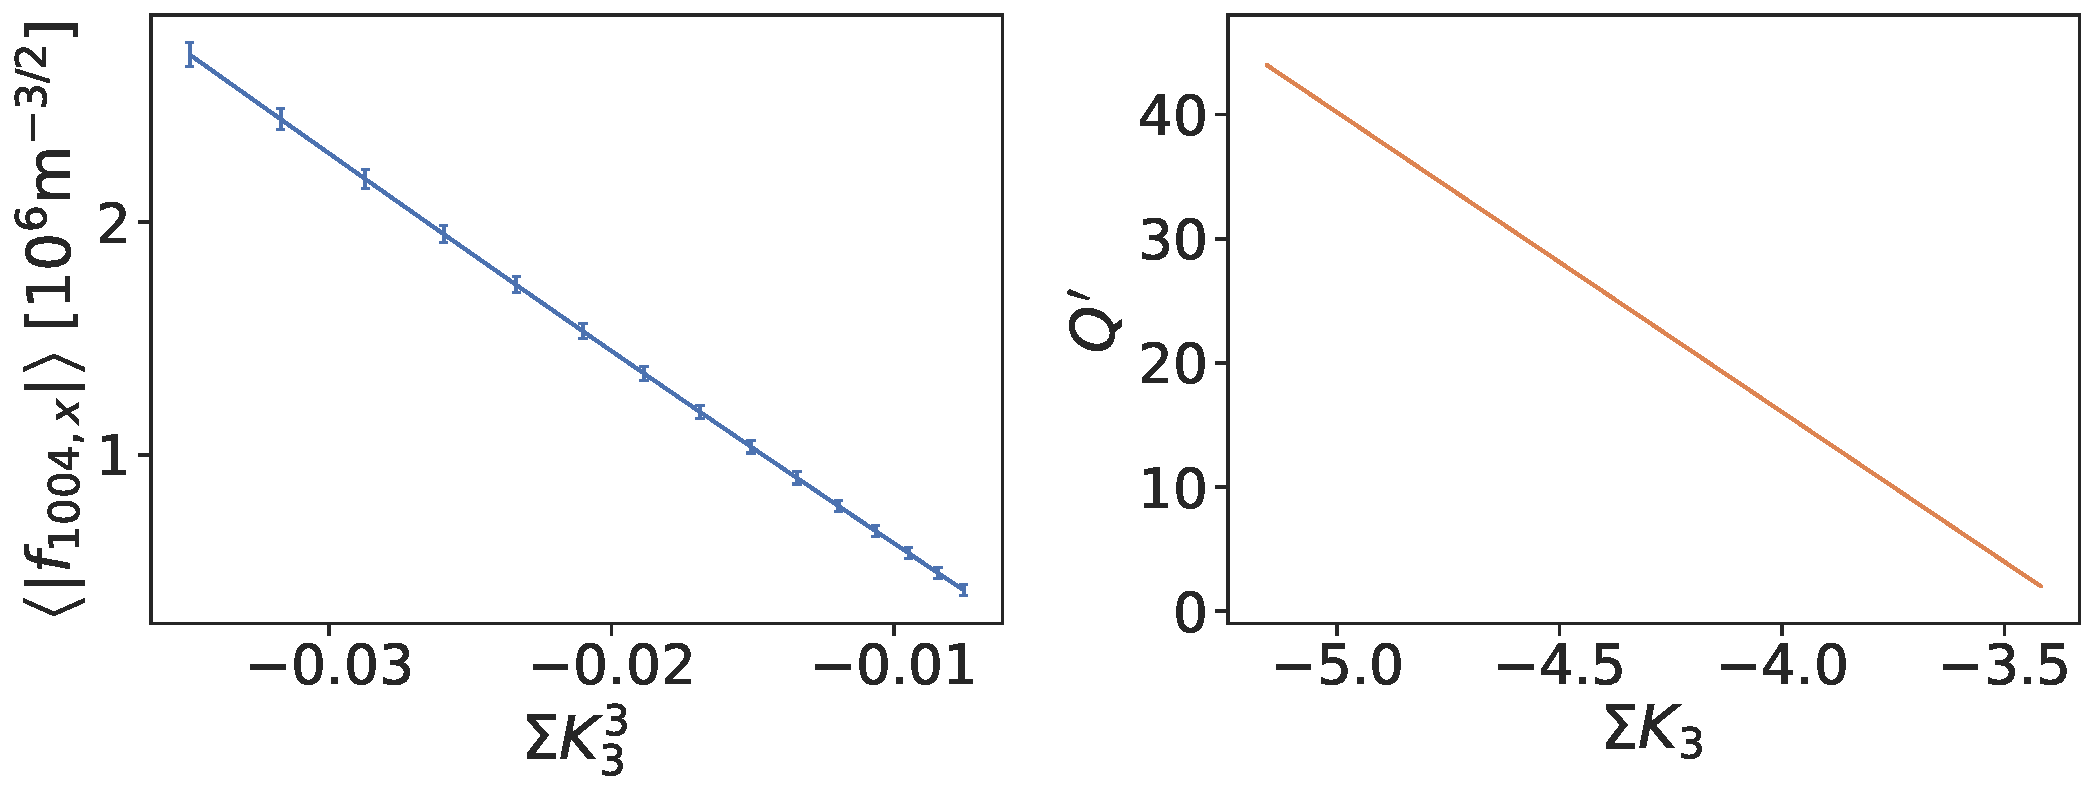
\includegraphics[width=0.9\textwidth]{./images/f1004/avg_f1004_k3.pdf}
    \caption{Average amplitude of the decapolar RDT $f_{1004}$ depending on the overall strength
    of the sextupoles used to control the linear chromaticity $Q'$. The right plot can be used
    to relate the RDT amplitude to a specific $Q'$ value.}
    \label{fig:decapoles:sextupoles_k3_f1004}
\end{figure}


To confirm what is observed in simulations, measurements were performed by varying $Q'$ and kicking
the beam with the AC-Dipole. Limited by losses, up to three measurements with distinct $Q'$ were
taken, as shows \cref{fig:decapoles:rdts:measured_f1004_from_sextupoles}.

\begin{figure}[!htb]
    \centering
    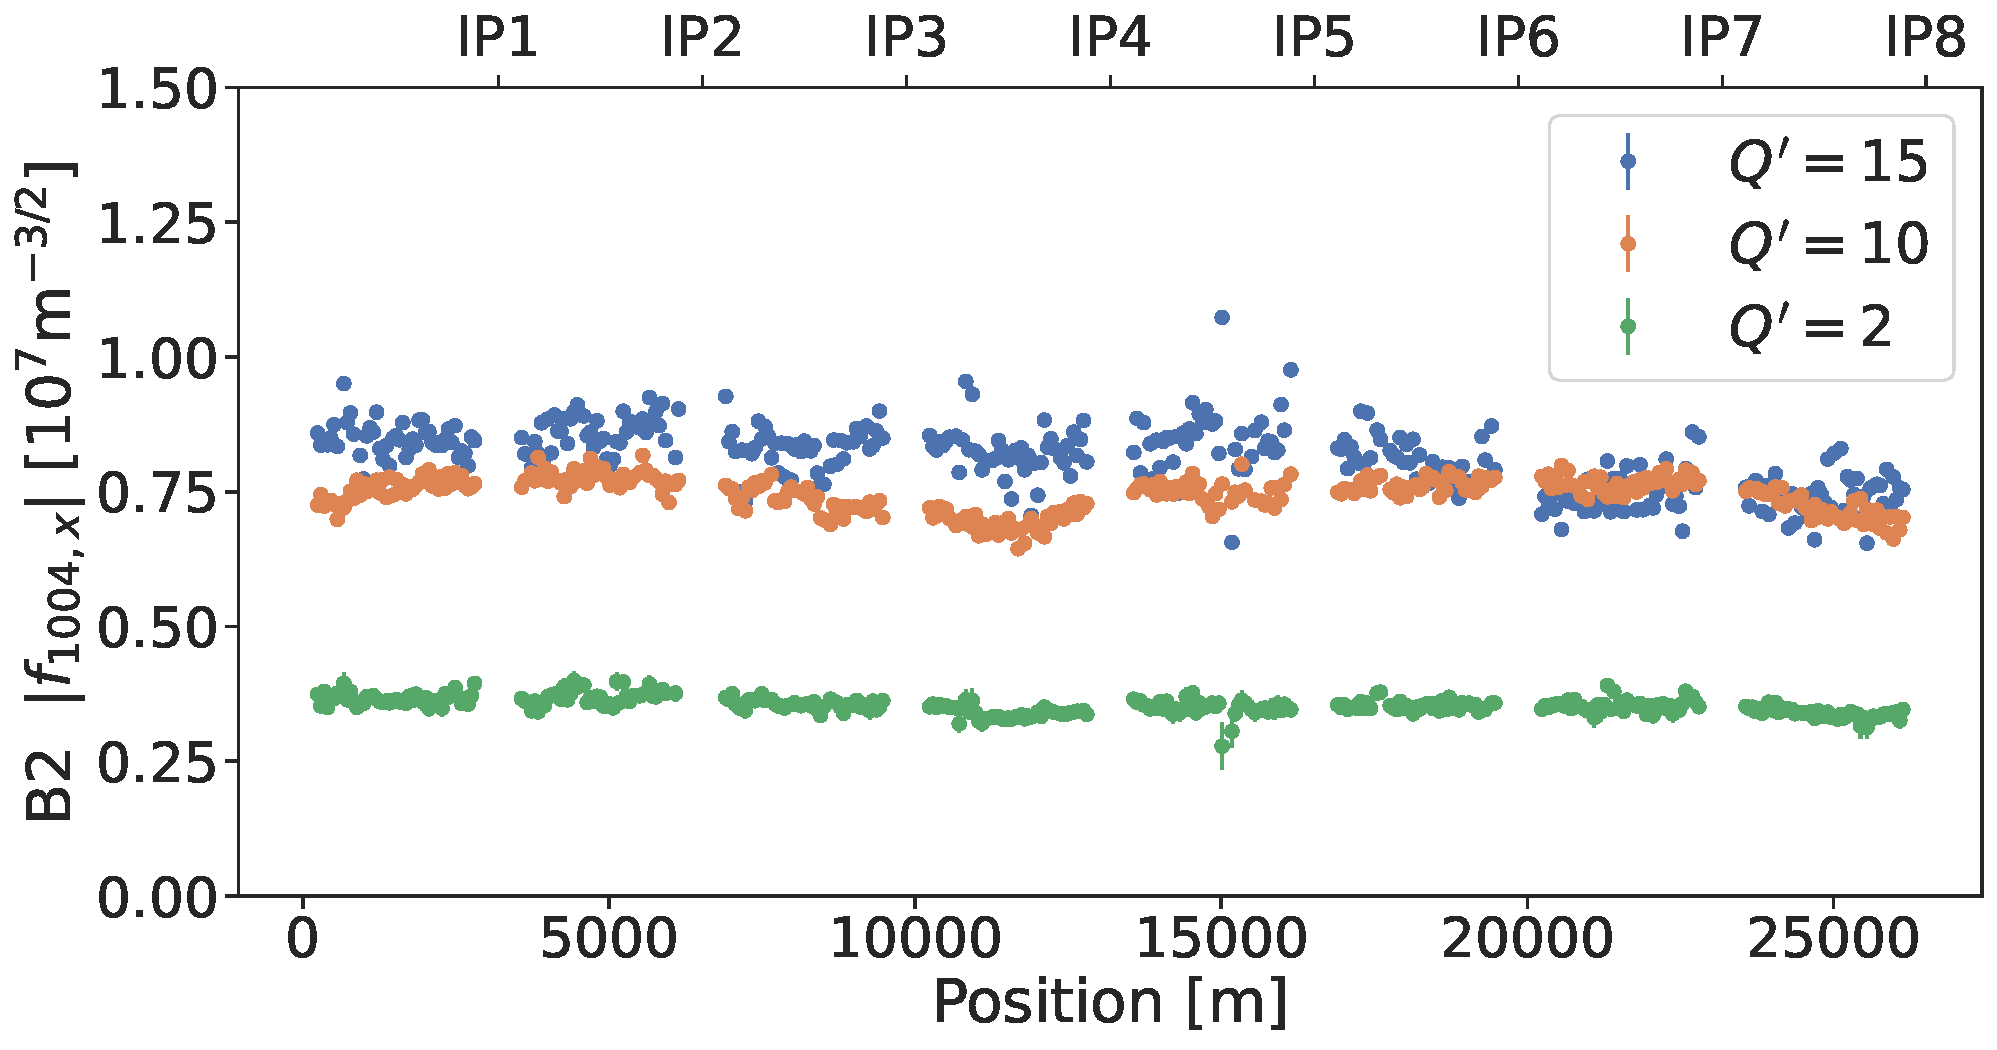
\includegraphics[width=0.85\textwidth]{./images/f1004/f1004x_q2_q10_q15.pdf}
    \caption{Measured change of the decapolar RDT $f_{1004}$ depending of the desired linear
    chromaticity $Q'$ generated by sextupoles. It is to be noted that the vertical axis is one
    order of magnitude higher than the previous simulations' plot.
    }
    \label{fig:decapoles:rdts:measured_f1004_from_sextupoles}
\end{figure}

Like in simulations, it is observed that an increase in $Q'$ translates to an increase in 
$|f_{1004}|$. The scale of the amplitude is though one order of magnitude higher than that of
simulations. An offset for all measurements could be explained by non-included field-errors. The
shift between them however should be similar between machine and simulations, this could be
due by the interaction of the sextupolar fields with octupoles, as detailed in the following
section. More data points with varying $Q'$ at similar kick amplitudes would be required to further
investigate.


% ------- Sextupole + Octupole ----------
\subsubsection{\review{Sextupoles and Octupoles}}


At the second order of the BCH expansion, the combination of a sextupole and an octupole yields a
decapolar-like expression.
Like sextupoles, octupoles are used in operation, thus contributing to decapolar fields. This
happens amongst other when correcting the second order chromaticity $Q''$ and most importantly with
the Landau Octupoles, which are powered to high strengths at injection energy to introduce Landau
damping~\cite{gareyte_landau_1997}.
Derivation of such a combination can be found in
\cref{appendix:transfer_map:sextupole_and_octupole}. The resulting Hamiltonian indeed is similar to
the terms of a decapole, dropping the $p_{x,y}$ terms for readability:

\begin{equation}
    \begin{aligned}
         H_3 H_4 &\propto \frac{1}{24} \left(x^5 + 2x^3y^2 + xy^4 \right)\\
                   &\sim    x^5 - 10x^3y^2 + 5xy^4.
    \end{aligned}
    \label{eq:decapoles:sextupole_octupole_b5}
\end{equation}

In order to assess the previous equation, simulations were run with several configurations.
As seen previously, a combination of two sextupoles creates a decapolar-like field, varying their 
field is thus not needed. Rather, a set of two configurations was run to check the impact of 
octupoles alone. The first configuration is ran with all sextupoles of the machine
turned off, while octupoles are powered. The second configuration turns off all sextupoles and
octupoles. \cref{fig:decapoles:rdts:sectupole_octupole_no_diff} shows the resulting RDT $f_{1004}$
from these simulations. It is there apparent that varying octupoles without sextupoles does not have 
any effect on this RDT.

\begin{figure}[!htb]
    \centering
    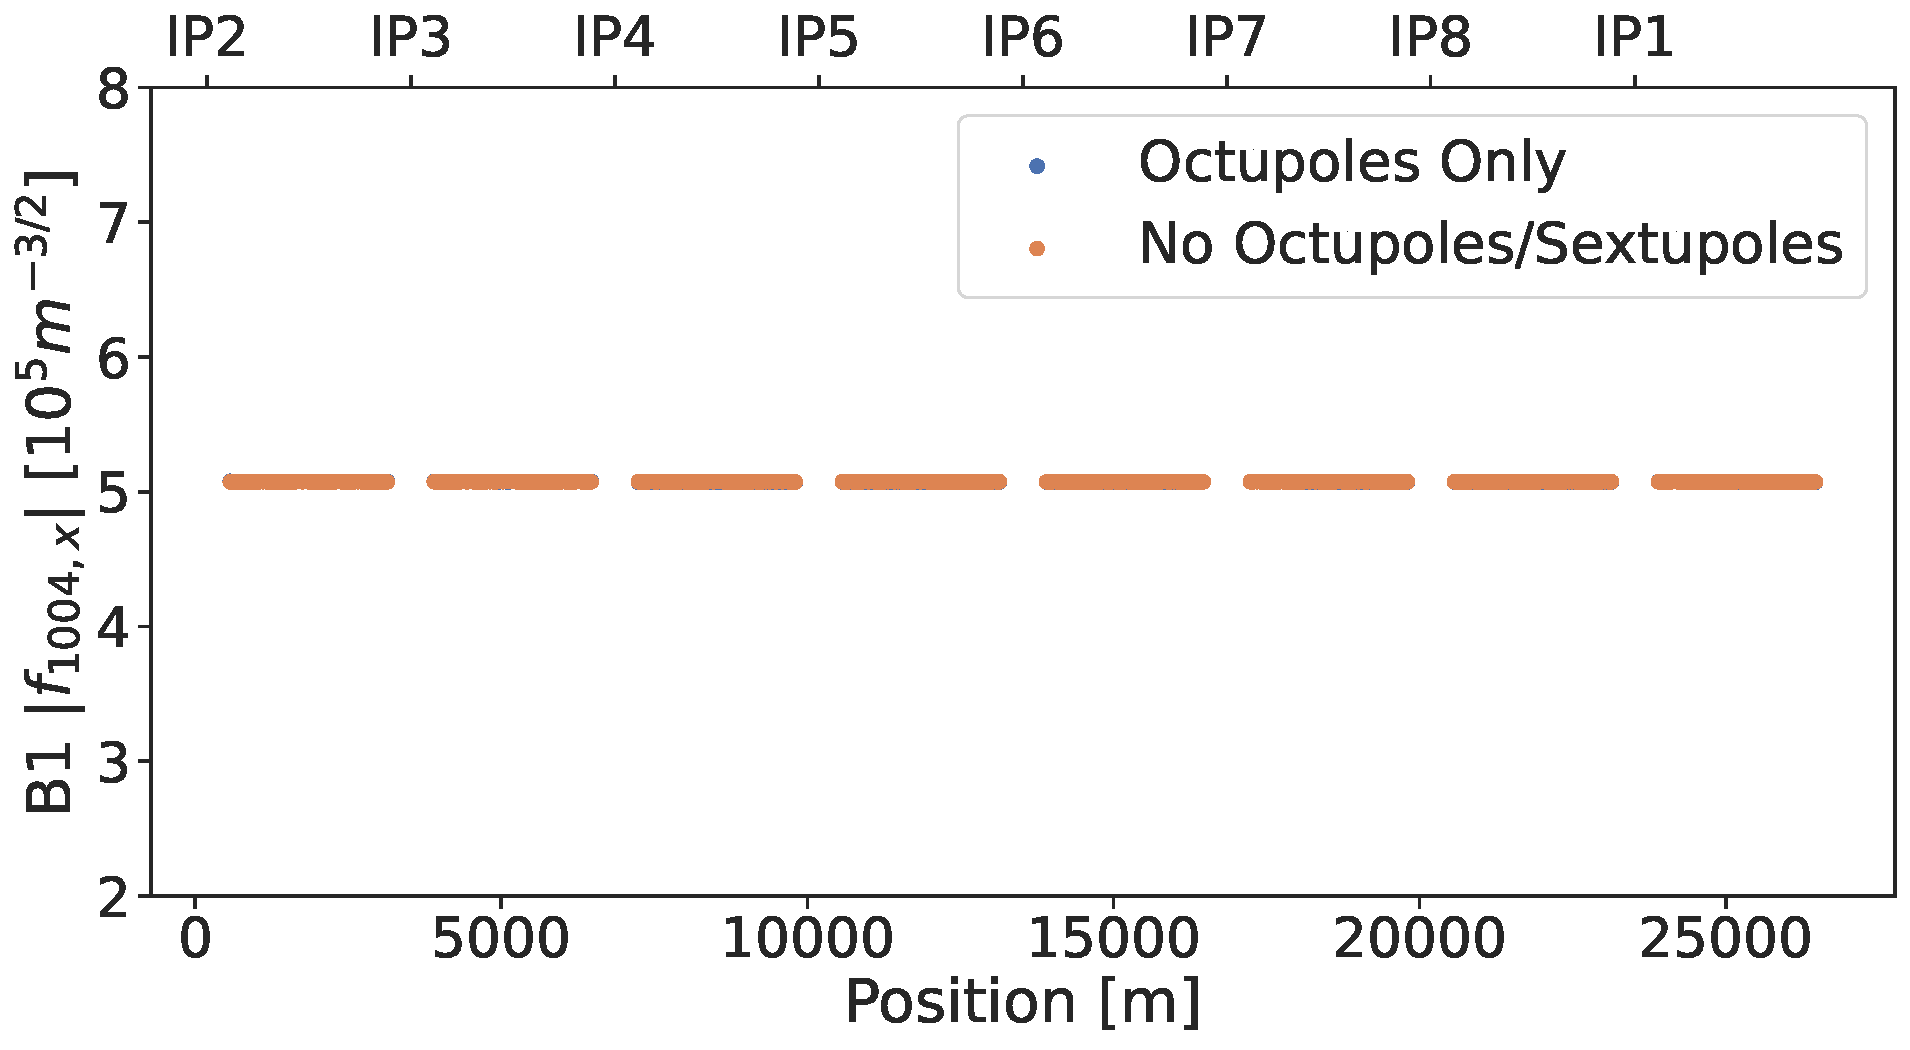
\includegraphics[width=0.8\textwidth]{./images/f1004/f1004_no_ms.pdf}
    \caption{Simulated decapolar RDT $f_{1004}$ with two different schemes. First scheme has
    lattice sextupoles turned off and octupoles turned on. Second scheme has all sextupoles of the
    lattice turned off and octupoles turned off as well. No difference is seen, as expected from
    the equations.}
    \label{fig:decapoles:rdts:sectupole_octupole_no_diff}
\end{figure}

The most powerful octupoles used in operation are the lattice octupoles, used for Landau damping.
\cref{fig:decapoles:rdts:simulation_mo_powered} shows a simulation ran with varying strengths of
those magnets. It can be noted here that the shift of the RDT is almost of an order of magnitude,
making octupoles a large contributor to the decapolar fields.

\begin{figure}[!htb]
    \centering
    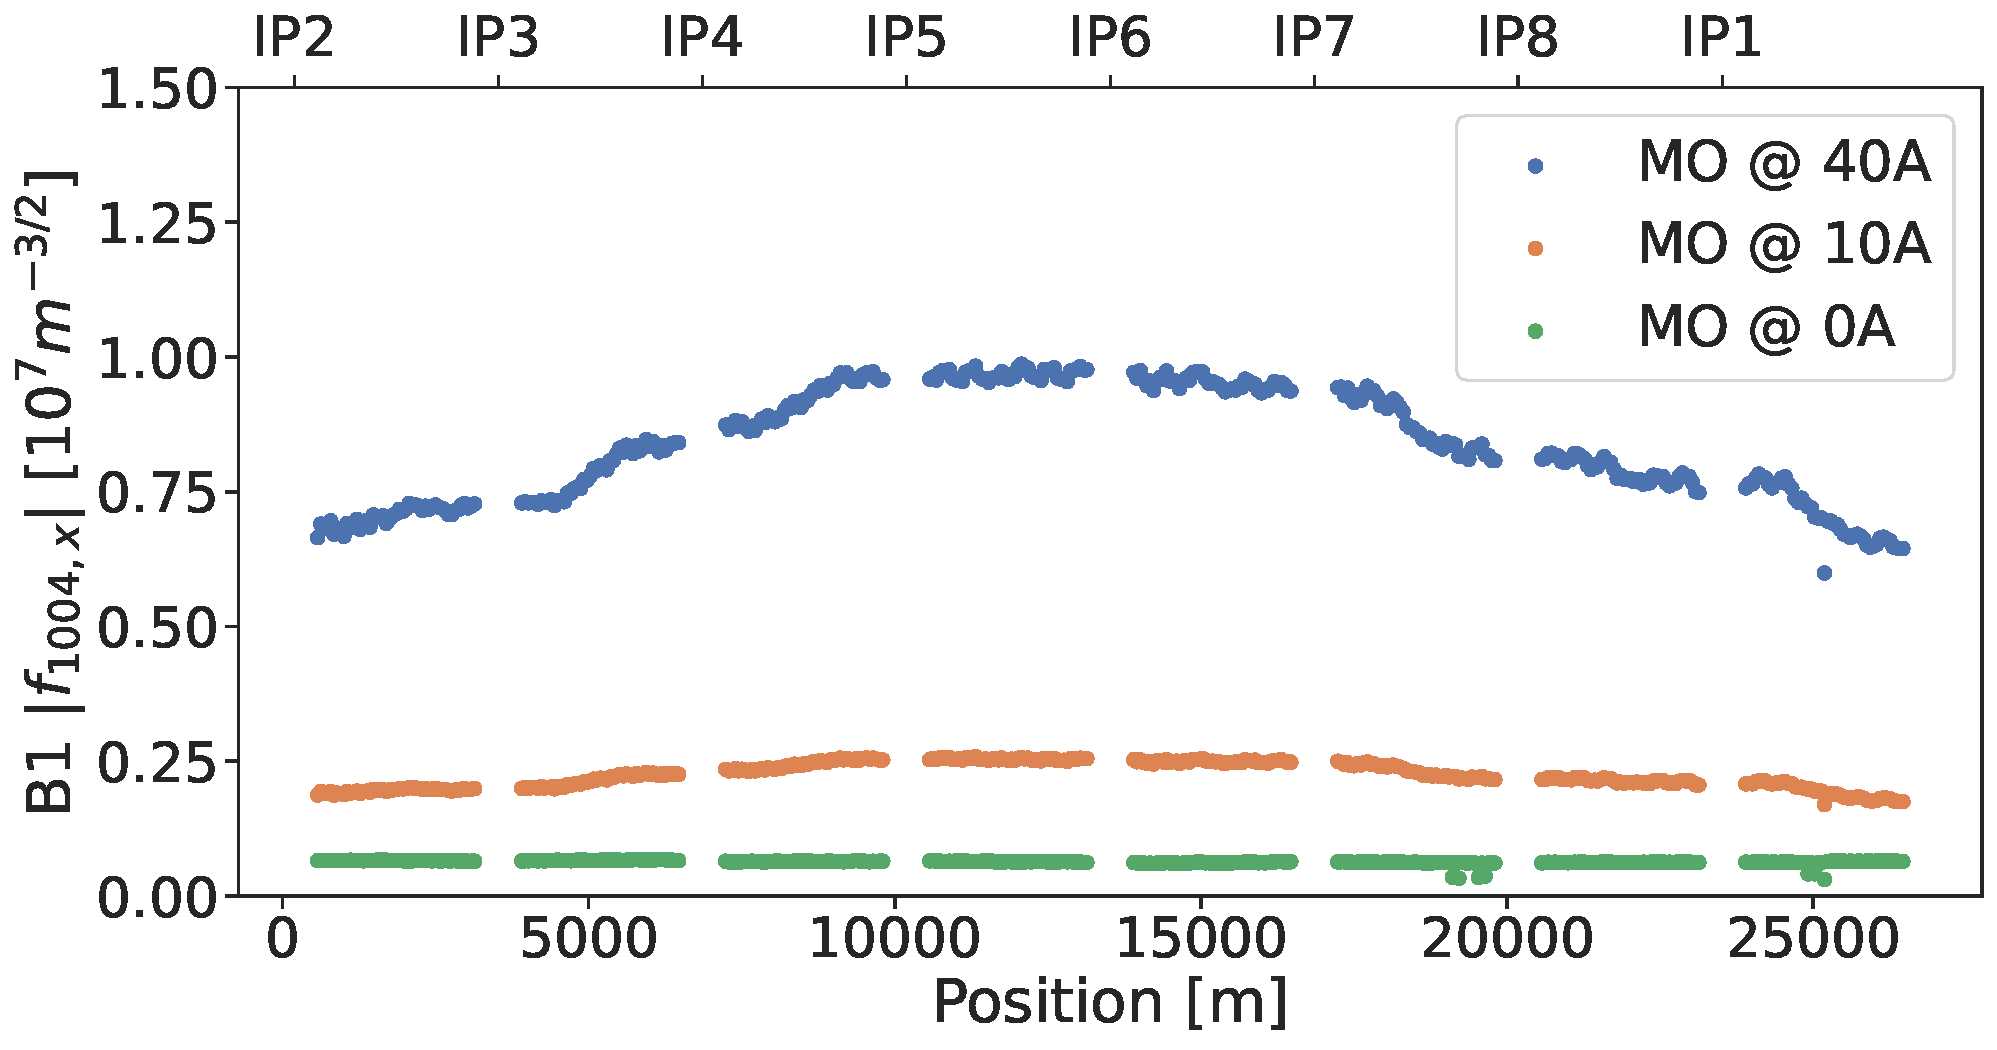
\includegraphics[width=0.8\textwidth]{./images/f1004/f1004_mo.pdf}
    \caption{Simulated change of the decapolar RDT $f_{1004}$ depending of the strength of the
    lattice octupoles used for Landau damping.}
    \label{fig:decapoles:rdts:simulation_mo_powered}
\end{figure}

While decapoles are expected to be the main contributors to decapolar fields, other strong sources
can indeed be identified. \cref{fig:decapoles:rdts:contributions} shows the average amplitude of the
RDT $f_{1004}$ depending on the error sources introduced in the simulations. A large contribution
comes from the octupolar errors in the main dipoles, being actually larger than the decapolar errors
in those magnets.

\begin{figure}[!htb]
    \centering
    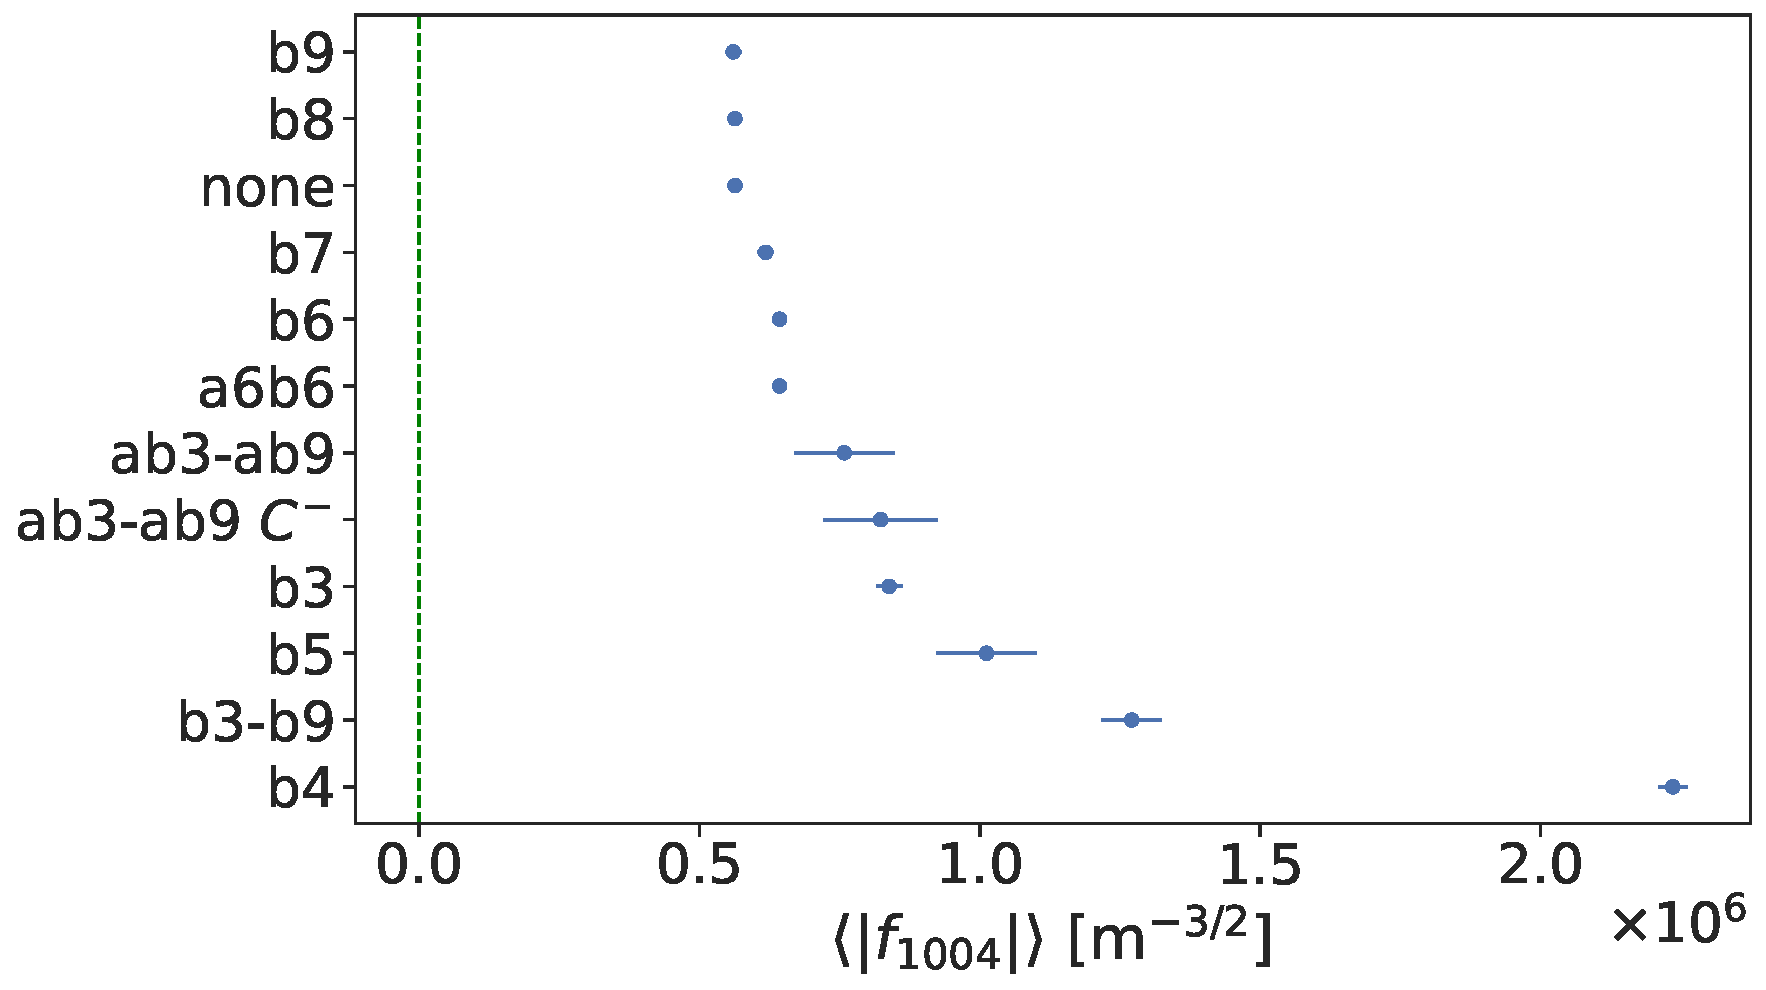
\includegraphics[width=0.8\textwidth]{./images/f1004/f1004_several_factors.pdf}
    \caption{Simulation of the amplitude of the decapolar RDT $f_{1004}$ depending on the field
             errors applied on main dipoles as well as coupling ($C^-$). While it is apparent that
             some multipolar errors drive the resonance higher, some combinations actually seem to
             cancel each other.}
    \label{fig:decapoles:rdts:contributions}
\end{figure}

\begin{wraptable}{r}{0.4\textwidth}
    \centering
    \begin{tabular}{rr}
    \toprule
    Factor & RMS $|f_{1004}|$ \\
    \midrule
       -10 & $37,308,159$         \\ 
        -4 &  $6,721,270$          \\ 
         0 &  $3,533,796$          \\ 
        -1 &  $2,333,384$          \\
    \bottomrule
    \end{tabular}
    \caption{RMS of $|f_{1004}|$ depending on the factor of the $Q''$ corrections.}
    \label{table:decapoles:corrections_dq2_f1004_rms}
\end{wraptable}

Measurements were performed to confirm and quantify the effect of octupoles coupled with sextupoles
on the decapolar fields. Previous corrections, aimed at correcting the second order chromaticity
$Q''$, via octupolar correctors \textit{MCO}, were applied with varying factors. Such corrections
apply use a uniform trim on all correctors of $\approx +2.5K_4$.
\cref{decapoles:rdts:measured_f1004_mco} shows a comparison of the resulting RDT with those
corrections at factors $-10$, $-4$, $-1$ and $0$.

\begin{figure}[!htb]
    \centering
    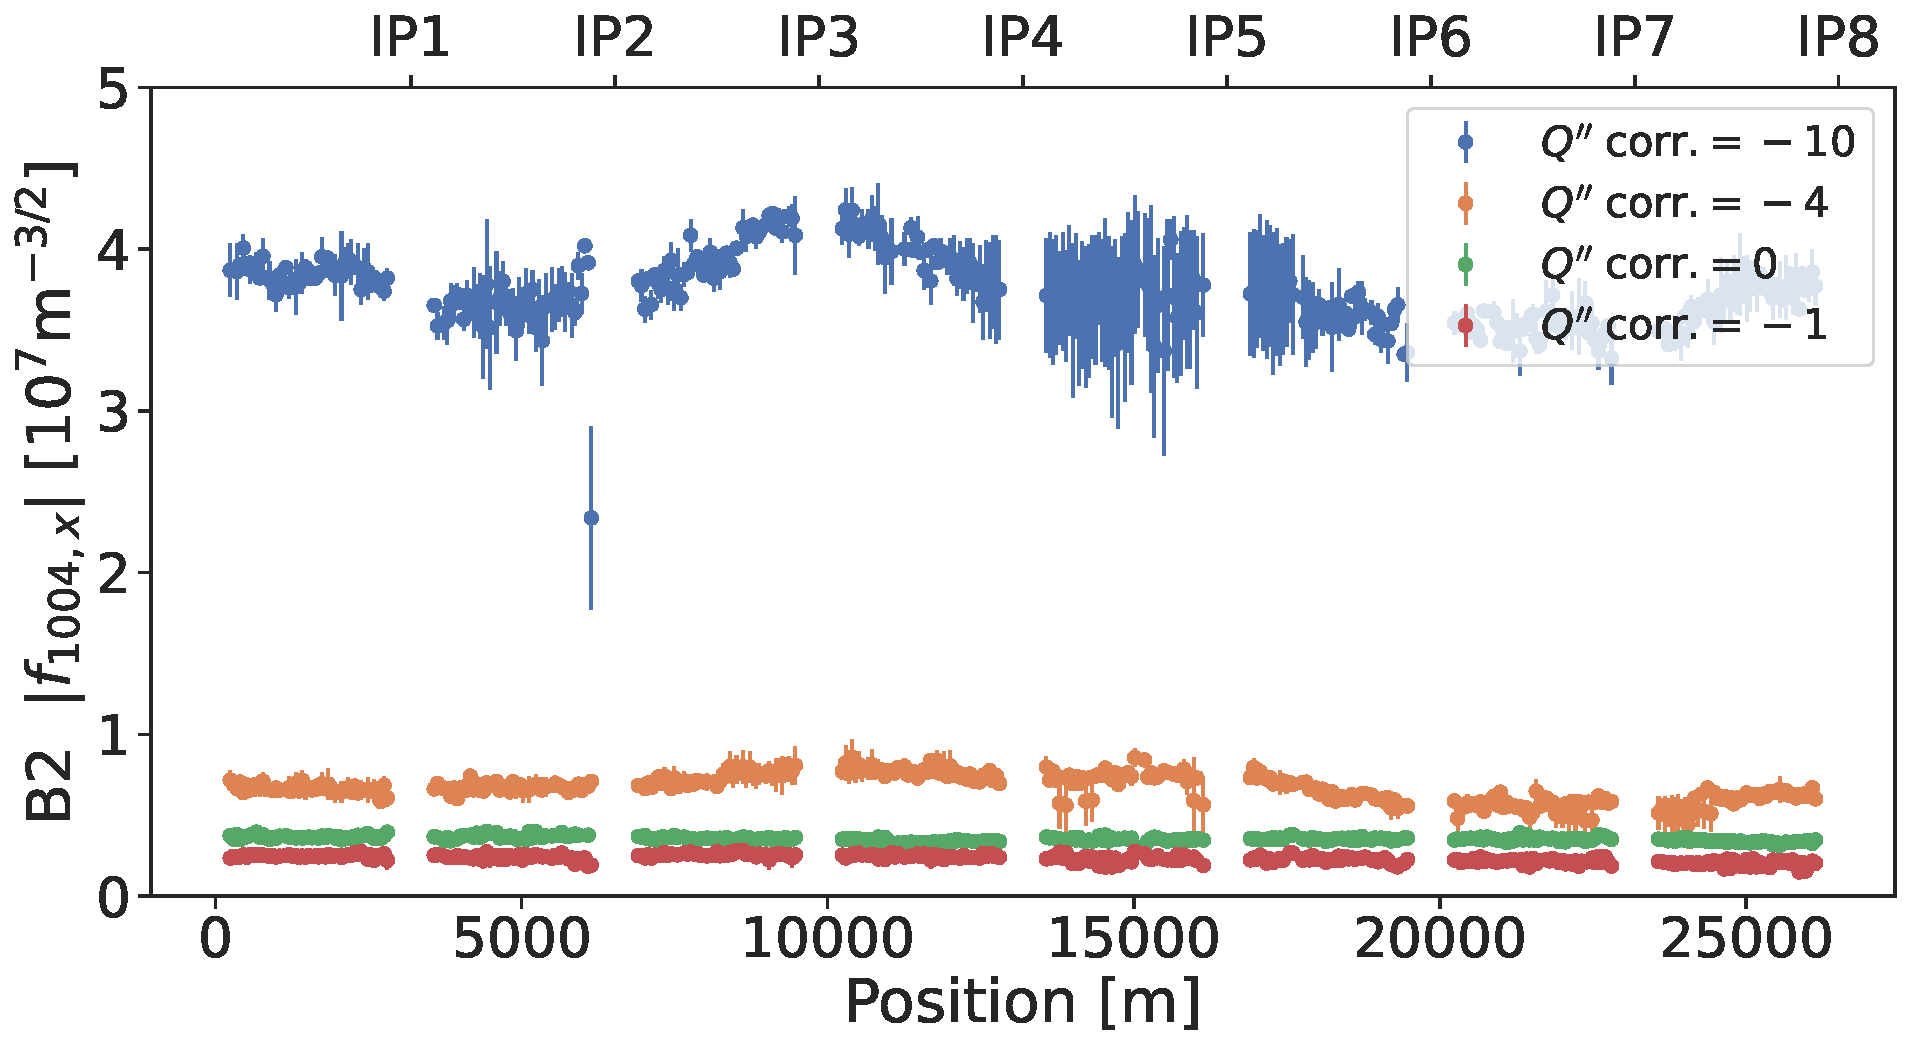
\includegraphics[width=0.8\textwidth]{./images/f1004/f1004x_mco_corr.pdf}
    \caption{Shift of the decapolar RDT $f_{1004}$ depending on the factor applied on octupolar
    corrections for $Q''$.}
    \label{decapoles:rdts:measured_f1004_mco}
\end{figure}


  
\cref{table:decapoles:corrections_dq2_f1004_rms} shows the RMS of the amplitude of this RDT for the 
various configurations. Similar to the shift observed when powering the landau octupoles in
simulations, the shift is of one order of magnitude between factors $-0$ and $-10$. Measurements
with landau octupoles were also attempted but losses made it impossible to obtain high enough
amplitudes to correctly measure the RDT.

Simulated and observed large shifts due tu octupoles are relevant to the operation of the LHC, as
resonances can be greatly deteriorated, especially when powering landau octupoles.
A better understanding of the interaction between Landau octupoles and octupolar correctors could
lead to improved corrections in not only octupolar but also decapolar fields in the future.